\documentclass[11pt,a4paper,twoside,openright]{book}

% ============================================================
% preambulo.tex — Estilo geral da apostila
% ============================================================

% ---- Fontes -------------------------------------------------
\usepackage{fontspec}
\setmainfont{Fira Sans}
\setsansfont{Fira Sans}
\setmonofont{Fira Mono}[Scale=0.88]

% ---- Idioma ---------------------------------------------------
\usepackage{polyglossia}
\setmainlanguage{brazilian}
\AtBeginDocument{
    \renewcommand{\tablename}{Tabela}
    \renewcommand{\figurename}{Figura}
    \renewcommand{\contentsname}{Sumário}
    \renewcommand{\appendixname}{Apêndice}
    \renewcommand{\chaptername}{Capítulo}
    \renewcommand{\partname}{Parte}
}

% ---- Layout de página ----------------------------------------
\usepackage[a4paper,margin=2.5cm,marginparwidth=2.2cm,marginparsep=0.4cm]{geometry}
\usepackage{setspace}
\onehalfspacing

% ---- Cores ------------------------------------------------
\usepackage{xcolor}
\definecolor{primaria}{HTML}{0B3D5C}      % azul petróleo escuro (título)
\definecolor{secundaria}{HTML}{12809E}    % azul-esverdeado (ESP32/PCB)
\definecolor{acento}{HTML}{E8762C}        % laranja circuito (destaques)
\definecolor{fundoclaro}{HTML}{F4F7F8}
\definecolor{fundocodigo}{HTML}{282C34}
\definecolor{textoclaro}{HTML}{E8EEF1}
\definecolor{cinzaesc}{HTML}{3B4750}
\definecolor{notaBg}{HTML}{EAF4F6}
\definecolor{notaBorda}{HTML}{12809E}
\definecolor{atencaoBg}{HTML}{FCEFE6}
\definecolor{atencaoBorda}{HTML}{E8762C}
\definecolor{dicaBg}{HTML}{EEF6EC}
\definecolor{dicaBorda}{HTML}{4C8C4A}

% ---- Matemática / símbolos ---------------------------------
\usepackage{amsmath,amssymb}

% ---- Gráficos e diagramas -----------------------------------
\usepackage{graphicx}
\usepackage{tikz}
\usetikzlibrary{shapes,arrows.meta,positioning,fit,backgrounds,calc}

% ---- Tabelas --------------------------------------------------
\usepackage{array,tabularx,booktabs,longtable,multirow}
\renewcommand{\arraystretch}{1.25}

% ---- Listas -----------------------------------------------
\usepackage{enumitem}
\setlist{itemsep=0.15em, topsep=0.4em}

% ---- Hyperlinks e referências -------------------------------
\usepackage{hyperref}
\hypersetup{
    colorlinks=true,
    linkcolor=primaria,
    citecolor=primaria,
    urlcolor=secundaria,
    pdftitle={Introdução à Linguagem C para Sistemas Embarcados},
    pdfauthor={Apostila EFB2006},
    pdfsubject={Linguagem C, ESP32, PlatformIO},
    bookmarksnumbered=true,
    bookmarksopen=true
}
\usepackage[capitalize,noabbrev]{cleveref}

% ---- Código-fonte (minted + tcolorbox) ------------------------
\usepackage{fontawesome5}
\usepackage{tcolorbox}
\tcbuselibrary{minted,breakable,skins}
\usemintedstyle{one-dark}

\tcbset{
  codigobase/.style={
    breakable, enhanced, listing only, minted style=one-dark,
    minted options={fontsize=\small, breaklines, breakanywhere,
                     tabsize=4, baselinestretch=1.05},
    colback=fundocodigo, colframe=fundocodigo,
    coltitle=textoclaro, fonttitle=\bfseries\ttfamily\small,
    boxrule=0pt, top=5mm, bottom=1mm, left=1mm, right=1mm,
    arc=2mm, outer arc=2mm,
    before={\color{textoclaro}},
    attach boxed title to top left={xshift=3mm, yshift=-1mm},
    boxed title style={colback=acento, arc=1.5mm, boxrule=0pt,
                        top=0.6mm, bottom=0.6mm, left=2mm, right=2mm},
  },
  terminalbase/.style={
    breakable, enhanced, listing only, minted style=one-dark,
    minted options={fontsize=\small, breaklines, breakanywhere,
                     tabsize=4, baselinestretch=1.05},
    colback=fundocodigo, colframe=cinzaesc,
    coltitle=textoclaro, fonttitle=\bfseries\ttfamily\small,
    boxrule=0.4pt, top=1mm, bottom=1mm, left=1mm, right=1mm,
    arc=2mm, outer arc=2mm,
    before={\color{textoclaro}},
  }
}

% Ambientes de código com título automático de arquivo
\newtcblisting{codigoc}[1]{codigobase, minted language=c, title={#1}}
\newtcblisting{codigoini}[1]{codigobase, minted language=ini, title={#1}}
\newtcblisting{codigobash}[1]{terminalbase, minted language=bash, title={#1}}

% ---- Caixas de destaque (nota, atenção, dica) -----------------
\newtcolorbox{nota}{
    breakable, enhanced, colback=notaBg, colframe=notaBorda,
    boxrule=0pt, leftrule=2.6pt, arc=1mm,
    left=3mm, right=3mm, top=1.5mm, bottom=1.5mm,
    fonttitle=\bfseries\color{notaBorda},
    title={\faInfoCircle\ \ Nota}
}
\newtcolorbox{atencao}{
    breakable, enhanced, colback=atencaoBg, colframe=atencaoBorda,
    boxrule=0pt, leftrule=2.6pt, arc=1mm,
    left=3mm, right=3mm, top=1.5mm, bottom=1.5mm,
    fonttitle=\bfseries\color{atencaoBorda},
    title={\faExclamationTriangle\ \ Atenção}
}
\newtcolorbox{dica}{
    breakable, enhanced, colback=dicaBg, colframe=dicaBorda,
    boxrule=0pt, leftrule=2.6pt, arc=1mm,
    left=3mm, right=3mm, top=1.5mm, bottom=1.5mm,
    fonttitle=\bfseries\color{dicaBorda},
    title={\faLightbulb\ \ Dica}
}
\newtcolorbox{esp32box}{
    breakable, enhanced, colback=fundoclaro, colframe=secundaria,
    boxrule=0pt, leftrule=2.6pt, arc=1mm,
    left=3mm, right=3mm, top=1.5mm, bottom=1.5mm,
    fonttitle=\bfseries\color{secundaria},
    title={\faMicrochip\ \ Aplicação no ESP32}
}

% ---- Títulos de capítulo/seção ---------------------------------
\usepackage{titlesec}
\titleformat{\chapter}[display]
  {\normalfont}
  {\Large\color{secundaria}\fontsize{14}{16}\selectfont\textsc{Capítulo \thechapter}}
  {6pt}
  {\Huge\bfseries\color{primaria}}
\titlespacing*{\chapter}{0pt}{-10pt}{28pt}

\titleformat{\section}
  {\normalfont\Large\bfseries\color{primaria}}
  {\thesection}{0.6em}{}
\titleformat{\subsection}
  {\normalfont\large\bfseries\color{secundaria}}
  {\thesubsection}{0.6em}{}
\titleformat{\subsubsection}
  {\normalfont\normalsize\bfseries\color{cinzaesc}}
  {\thesubsubsection}{0.6em}{}

% ---- Cabeçalhos e rodapés -------------------------------------
\usepackage{fancyhdr}
\pagestyle{fancy}
\fancyhf{}
\renewcommand{\headrulewidth}{0.4pt}
\renewcommand{\footrulewidth}{0pt}
\fancyhead[LE,RO]{\small\thepage}
\fancyhead[RE]{\small\color{cinzaesc}\nouppercase{\leftmark}}
\fancyhead[LO]{\small\color{cinzaesc}\nouppercase{\rightmark}}

\fancypagestyle{plain}{
  \fancyhf{}
  \fancyhead[LE,RO]{\small\thepage}
  \renewcommand{\headrulewidth}{0pt}
}

% Páginas em branco (inseridas para iniciar capítulos em página ímpar)
% não devem exibir cabeçalho.
\makeatletter
\renewcommand{\cleardoublepage}{%
  \clearpage
  \if@twoside
    \ifodd\c@page\else
      \hbox{}\thispagestyle{empty}\newpage
      \if@twocolumn\hbox{}\newpage\fi
    \fi
  \fi
}
\makeatother

% ---- Sumário -----------------------------------------------
\usepackage{tocloft}
\renewcommand{\cftchapfont}{\bfseries\color{primaria}}
\renewcommand{\cftchappagefont}{\color{primaria}}
\renewcommand{\cftsecfont}{\color{cinzaesc}}

% ---- Numeração de código e legendas ---------------------------
\usepackage{caption}
\captionsetup{font=small,labelfont={bf,color=primaria}}

% ---- Comando utilitário para inline code ------------------
\newcommand{\code}[1]{\texttt{\color{secundaria}#1}}
\newcommand{\ESP}{ESP32\xspace}
\usepackage{xspace}


\title{Introdução à Linguagem C para Sistemas Embarcados}
\author{Apostila EFB2006}
\date{\today}

\begin{document}

% ============================================================
% capa.tex — Página de rosto
% ============================================================
\begin{titlepage}
\newgeometry{margin=0cm}
\pagecolor{primaria}
\begin{tikzpicture}[remember picture, overlay]
    % --- trilhas de circuito decorativas ---
    \begin{scope}[white, opacity=0.10, line width=1.4pt]
        \draw (2,-3) -- (2,-6) -- (5,-6) -- (5,-9);
        \draw (3,-3) -- (3,-4.5) -- (7,-4.5);
        \draw (16,-2) -- (16,-5) -- (13,-5) -- (13,-8);
        \draw (17.5,-3) -- (17.5,-7) -- (15,-7);
        \draw (1,-20) -- (1,-17) -- (4,-17);
        \draw (18,-24) -- (18,-21) -- (15,-21) -- (15,-19);
        \foreach \p in {(2,-3),(5,-6),(5,-9),(3,-3),(7,-4.5),
                         (16,-2),(13,-5),(13,-8),(17.5,-3),(15,-7),
                         (1,-20),(4,-17),(18,-24),(15,-19)}
            \fill \p circle (2.2pt);
    \end{scope}

    % --- chip / microcontrolador estilizado (canto inferior direito) ---
    \begin{scope}[shift={(15.3,-25.2)}, secundaria]
        \fill[opacity=0.9] (0,0) rectangle (3.4,3.4);
        \foreach \i in {0,...,6} {
            \draw[white, opacity=0.9, line width=0.9pt] (0.4+\i*0.45,3.4) -- (0.4+\i*0.45,3.9);
            \draw[white, opacity=0.9, line width=0.9pt] (0.4+\i*0.45,0) -- (0.4+\i*0.45,-0.5);
            \draw[white, opacity=0.9, line width=0.9pt] (0,0.4+\i*0.45) -- (-0.5,0.4+\i*0.45);
            \draw[white, opacity=0.9, line width=0.9pt] (3.4,0.4+\i*0.45) -- (3.9,0.4+\i*0.45);
        }
        \node[white, font=\footnotesize\bfseries\ttfamily] at (1.7,1.7) {ESP32};
    \end{scope}

    % --- faixa de acento ---
    \fill[acento] (0,-8.6) rectangle (21,-8.85);
\end{tikzpicture}

\begin{tikzpicture}[remember picture, overlay]
    \node[anchor=north west, text width=15cm, align=left, xshift=2cm, yshift=-3.2cm] at (current page.north west)
        {\color{textoclaro}\fontsize{11}{13}\selectfont\textsc{Apostila Didática}};

    \node[anchor=north west, text width=16.5cm, align=left, xshift=2cm, yshift=-4.3cm] at (current page.north west)
        {\color{white}\fontsize{34}{40}\selectfont\bfseries Introdução à Linguagem C\\[2pt] para Sistemas Embarcados};

    \node[anchor=north west, text width=15cm, align=left, xshift=2cm, yshift=-9.9cm] at (current page.north west)
        {\color{acento}\fontsize{15}{18}\selectfont\bfseries Programação do ESP32 com o PlatformIO};

    \node[anchor=north west, text width=13cm, align=left, xshift=2cm, yshift=-11.1cm] at (current page.north west)
        {\color{textoclaro}\fontsize{11}{15}\selectfont
         Dos fundamentos da linguagem C à programação\\de sistemas embarcados.};

    \node[anchor=south west, xshift=2cm, yshift=2.2cm] at (current page.south west)
        {\color{textoclaro}\fontsize{10}{12}\selectfont\ttfamily EFB2006 \textbullet\ \the\year};

    \node[anchor=south west, xshift=2cm, yshift=4.6cm] at (current page.south west)
        {
\includegraphics[width=4cm]{imagens/logo.png}};
\end{tikzpicture}
\end{titlepage}
\restoregeometry
\nopagecolor
\clearpage


\frontmatter
\chapter*{Prefácio}
\addcontentsline{toc}{chapter}{Prefácio}
\markboth{Prefácio}{Prefácio}

Esta apostila foi escrita para quem está dando os primeiros passos em programação e, ao mesmo tempo, quer entender \emph{para onde} esses passos levam quando o assunto é \textbf{sistemas embarcados}. Em vez de tratar a linguagem C como um fim em si mesma — como costuma acontecer em cursos introdutórios genéricos —, cada conceito aqui apresentado é conduzido com um destino em mente: o controle de um microcontrolador real, o \textbf{ESP32}, programado através do ambiente \textbf{PlatformIO}.

\section*{Por que C e por que o ESP32?}

A linguagem C continua sendo, décadas após sua criação, a linguagem mais próxima do hardware que ainda é acessível a iniciantes. Ela expõe conceitos que linguagens de alto nível escondem — como a organização da memória, o tamanho exato de cada tipo de dado e a manipulação direta de endereços — e é exatamente esse tipo de controle que se exige ao programar um microcontrolador, onde os recursos de memória e processamento são limitados e cada byte importa.

O ESP32 foi escolhido como plataforma de referência por ser barato, extremamente popular, bem documentado e por reunir em um único chip um processador dual-core, Wi-Fi, Bluetooth e uma quantidade generosa de periféricos (GPIOs, conversores analógico-digitais, saídas PWM, interfaces de comunicação serial). Isso permite que, com poucas linhas de código C, o estudante veja resultados físicos e imediatos: um LED que acende, um sensor que responde, um motor que gira.

\section*{Como este material está organizado}

A apostila é dividida em duas partes:

\begin{itemize}
    \item \textbf{Parte I — Fundamentos da Linguagem C:} cobre a sintaxe, os tipos de dados, as estruturas de controle, funções, arranjos, ponteiros, alocação de memória e organização de código em múltiplos arquivos. Os exemplos desta parte rodam tanto em um computador comum (compilados com \code{gcc}) quanto, quando fizer sentido, diretamente no ESP32.
    \item \textbf{Parte II — Sistemas Embarcados com o ESP32 e o PlatformIO:} apresenta o ambiente de desenvolvimento PlatformIO, a arquitetura do ESP32 e o uso de seus periféricos — entradas e saídas digitais, PWM, conversão analógico-digital, comunicação serial, interrupções e temporizadores — sempre com projetos completos e funcionais.
\end{itemize}

Ao longo dos capítulos você encontrará três tipos de caixas de destaque:

\begin{nota}
Informações complementares que aprofundam ou contextualizam o conceito tratado.
\end{nota}

\begin{dica}
Sugestões práticas, atalhos e boas práticas de programação.
\end{dica}

\begin{atencao}
Armadilhas comuns e erros frequentes — vale a pena prestar atenção especial aqui.
\end{atencao}

\section*{O que você vai precisar}

\begin{itemize}
    \item Um computador com \href{https://code.visualstudio.com/}{Visual Studio Code} e a extensão \textbf{PlatformIO IDE} instalada (o \cref{cap:platformio} explica o processo completo);
    \item Uma placa de desenvolvimento com o chip \textbf{ESP32} (qualquer variante — DevKit, WROOM, WROVER — e um cabo USB compatível);
    \item Curiosidade para errar, compilar de novo e tentar outra vez — é assim que se aprende a programar.
\end{itemize}

Bons estudos!

\newpage

\tableofcontents

\mainmatter

\part{Fundamentos da Linguagem C}
\chapter{Primeiros Passos}
\label{cap:primeiros-passos}

C é uma linguagem de programação criada no início dos anos 1970 por Dennis Ritchie, nos laboratórios da Bell, originalmente para reescrever o sistema operacional Unix. Mais de cinquenta anos depois, ela continua sendo uma das linguagens mais usadas do mundo — e isso não é acidente: C oferece um equilíbrio raro entre abstração suficiente para ser produtiva e proximidade suficiente do hardware para ser eficiente. É exatamente por esse motivo que praticamente todo sistema operacional, driver de dispositivo e firmware de microcontrolador — incluindo o do \ESP{} — tem C em algum lugar de sua base.

\begin{nota}
A linguagem C é \textbf{compilada}: o código-fonte que escrevemos (extensão \code{.c}) é traduzido por um programa chamado \textbf{compilador} para linguagem de máquina antes de ser executado. Isso é diferente de linguagens \textbf{interpretadas}, como Python ou JavaScript, cujo código é lido e executado linha a linha por um interpretador em tempo de execução. Java fica no meio do caminho: compila para um bytecode intermediário, interpretado depois pela JVM. Essa distinção será retomada no \cref{cap:sistemas-numericos}, quando falarmos sobre o processo de compilação em detalhe.
\end{nota}

\section{O primeiro programa}

Por tradição — que remonta ao próprio livro de Kernighan e Ritchie sobre a linguagem —, o primeiro programa que qualquer pessoa escreve em C é o "\emph{Hello, World!}": um programa que apenas exibe essa mensagem na tela.

\begin{codigoc}{hello\_world.c}
/*
    Seu primeiro programa em C
    ** Para dar sorte! **
*/

#include <stdio.h>          // Inclui a biblioteca padrao de
                            // entrada e saida (Standard Input/Output)

int main(void) {

    printf("Hello, World!\n");   // Exibe "Hello, World!" na tela
    return 0;

}
\end{codigoc}

Apesar de simples, este programa já contém quase todos os elementos estruturais que qualquer programa em C possui. Vamos destrinchá-lo peça por peça.

\subsection{Comentários}

As primeiras linhas do código são um comentário de múltiplas linhas, delimitado por \code{/*} e \code{*/}. Mais adiante, na mesma linha do \code{\#include}, aparece um comentário de linha única, iniciado por \code{//} e válido até o final da linha.

\begin{codigoc}{Sintaxe de comentários}
/*
    Este e' um comentario de multiplas linhas.
    Pode ocupar quantas linhas forem necessarias.
*/

// Este e' um comentario de uma unica linha.
\end{codigoc}

Comentários são trechos de texto totalmente ignorados pelo compilador — eles existem apenas para quem lê o código. Use-os para explicar \emph{por que} uma decisão foi tomada, não para descrever o óbvio.

\subsection{A diretiva \code{\#include}}

A linha \code{\#include <stdio.h>} não é, tecnicamente, um comando C: é uma \textbf{diretiva de pré-processador}, processada \emph{antes} da compilação propriamente dita. Ela instrui o compilador a inserir, naquele ponto do arquivo, o conteúdo do arquivo de cabeçalho (\emph{header}) \code{stdio.h}, que declara as funções da biblioteca padrão de entrada e saída — entre elas, a função \code{printf} usada logo abaixo. O pré-processador e as bibliotecas de software serão tratados com mais profundidade no \cref{cap:modularizacao}.

\subsection{A função \code{main}}

Todo programa C possui exatamente um ponto de entrada: a função \code{main}. É a partir dela que a execução do programa começa.

\begin{codigoc}{Assinatura da função main}
int main(void) {
    // ... corpo do programa ...
}
\end{codigoc}

\begin{itemize}
    \item O \code{int} antes de \code{main} indica que essa função \textbf{retorna} um número inteiro ao sistema operacional quando termina — o chamado \emph{código de saída};
    \item O \code{void} entre parênteses indica que, neste caso, a função não recebe parâmetros de entrada. É possível receber argumentos de linha de comando aqui, assunto tratado mais adiante no material;
    \item Tudo o que está entre as chaves \code{\{ \}} constitui o \textbf{corpo} (ou escopo) da função — o bloco de instruções que será executado.
\end{itemize}

\subsection{A instrução \code{printf}}

\code{printf} (\emph{print formatted}) é uma função da biblioteca \code{stdio.h} responsável por exibir texto na saída padrão — normalmente, o terminal. O texto entre aspas duplas é uma \textbf{string} (uma sequência de caracteres); a sequência \code{\textbackslash n} dentro dela é um \textbf{caractere de escape} que representa uma quebra de linha. Formatação de entrada e saída de dados é aprofundada no \cref{cap:entrada-saida}.

\subsection{O retorno e o ponto e vírgula}

A última instrução, \code{return 0;}, encerra a execução de \code{main} devolvendo o valor \code{0} ao sistema operacional — por convenção, \code{0} significa ``o programa terminou sem erros''. Qualquer outro valor costuma indicar algum tipo de falha. Esse conceito é fundamental em engenharia de software: é assim que um programa comunica sucesso ou falha para quem o executou (outro programa, um script, ou o próprio sistema operacional).

Repare também que \textbf{toda instrução em C termina com ponto e vírgula} (\code{;}). Esquecer esse detalhe é, disparadamente, o erro de sintaxe mais comum entre iniciantes.

\begin{atencao}
O compilador C é implacável com pequenos deslizes de sintaxe: uma chave não fechada, um ponto e vírgula esquecido ou um parêntese a mais são suficientes para impedir a compilação inteira do programa. Leia as mensagens de erro com atenção — elas quase sempre indicam a linha exata (ou próxima dela) onde o problema ocorre.
\end{atencao}

\section{Compilando e executando}

Para transformar o arquivo \code{hello\_world.c} em um programa executável, usamos um compilador. No Linux e no macOS, o mais comum é o \textbf{GCC} (\emph{GNU Compiler Collection}); no Windows, alternativas como MinGW ou o compilador do próprio Visual Studio cumprem o mesmo papel.

\begin{codigobash}{Compilando com gcc}
$ gcc -o hello_world hello_world.c
\end{codigobash}

O parâmetro \code{-o hello\_world} define o nome do arquivo executável gerado. Sem ele, o GCC produziria um arquivo chamado \code{a.out} por padrão. Para executar o programa:

\begin{codigobash}{Executando o programa}
$ ./hello_world
Hello, World!
\end{codigobash}

\begin{dica}
No Linux/macOS, o \code{./} antes do nome do executável é necessário porque, por segurança, o diretório atual normalmente não faz parte do \code{PATH} do sistema — sem ele, o shell não saberia onde procurar o programa.
\end{dica}

\section{E no ESP32?}

Um microcontrolador como o \ESP{} não tem teclado, tela ou sistema operacional convencional — então não existe um terminal esperando por \code{Hello, World!}. Ainda assim, o princípio é idêntico: escrevemos código C, ele é compilado, e o resultado (um arquivo \emph{binário}) é carregado para a memória do dispositivo, onde passa a ser executado assim que ele é ligado.

\begin{esp32box}
No mundo dos microcontroladores, o equivalente ao \emph{Hello, World!} costuma ser o \textbf{blink}: piscar um LED. É o primeiro programa que qualquer pessoa escreve para o \ESP{}, porque prova visualmente que o código foi compilado, carregado e está de fato em execução no hardware. Chegaremos lá: a partir do \cref{cap:platformio}, vamos configurar o ambiente PlatformIO e, no \cref{cap:gpio}, escrever exatamente esse programa.

Por enquanto, a diferença mais importante a guardar é esta: em vez de uma única função \code{main} que roda uma vez e termina, um firmware embarcado tipicamente gira em torno de um \textbf{laço infinito} — o programa nunca ``termina'' (não haveria sentido em um \code{return} para o quê, exatamente?), ele fica reagindo a eventos e atualizando o estado do sistema enquanto houver energia. No framework que usaremos (Arduino, via PlatformIO), isso aparece de forma bem explícita: em vez de uma função \code{main}, escreveremos duas funções, \code{setup()} e \code{loop()} — a segunda chamada repetidamente, para sempre, pelo próprio framework.
\end{esp32box}

Toda a Parte I desta apostila usa o \code{gcc} e a execução em um computador comum como ambiente de aprendizado, exatamente porque isso permite testar cada conceito de forma rápida e isolada, sem depender de hardware específico. Os mesmos conceitos — tipos de dados, estruturas de controle, funções, ponteiros — são diretamente aplicáveis ao firmware do \ESP{} que construiremos na Parte II.

\chapter{Sistemas Numéricos, Memória e Compilação}
\label{cap:sistemas-numericos}

Antes de avançar pela sintaxe da linguagem, vale entender melhor o terreno sobre o qual ela é construída: como um computador representa números, como organiza a memória e o que, de fato, acontece entre escrever um arquivo \code{.c} e obter um programa executável. Esses fundamentos são especialmente relevantes em sistemas embarcados, onde memória é escassa e o programador frequentemente manipula dados diretamente em binário e hexadecimal.

\section{Sistema binário}

Computadores armazenam e processam informação usando apenas dois estados elétricos — ligado e desligado —, representados matematicamente pelos dígitos \(0\) e \(1\). Esse é o \textbf{sistema binário} (base 2). Cada dígito binário é chamado de \textbf{bit} (\emph{binary digit}); um grupo de 8 bits forma um \textbf{byte}.

Um número binário é interpretado da mesma forma que um número decimal, mas com potências de 2 em vez de potências de 10:

\[
1011_2 = 1\times2^3 + 0\times2^2 + 1\times2^1 + 1\times2^0 = 8+0+2+1 = 11_{10}
\]

\begin{table}[h]
\centering
\begin{tabular}{@{}cccc@{}}
\toprule
\textbf{Bits} & \textbf{Nome} & \textbf{Valores possíveis} & \textbf{Intervalo (sem sinal)} \\
\midrule
1 & bit      & 2         & 0 a 1 \\
4 & nibble   & 16        & 0 a 15 \\
8 & byte     & 256       & 0 a 255 \\
16 & word (na maioria dos MCUs de 16b) & 65\,536 & 0 a 65\,535 \\
32 & double word & 4\,294\,967\,296 & 0 a $2^{32}-1$ \\
\bottomrule
\end{tabular}
\caption{Grupos comuns de bits e sua capacidade de representação.}
\end{table}

\section{Sistemas octal e hexadecimal}

Escrever endereços de memória ou máscaras de bits inteiramente em binário é verboso e propenso a erros. Por isso, é comum usar bases que sejam potências de 2 e que reduzam o número de dígitos: o \textbf{octal} (base 8) e, principalmente, o \textbf{hexadecimal} (base 16).

No hexadecimal, os dígitos vão de 0 a 9 e depois de A a F (representando 10 a 15). Cada dígito hexadecimal representa exatamente 4 bits (um nibble), o que torna a conversão entre binário e hexadecimal praticamente mecânica:

\begin{table}[h]
\centering
\begin{tabular}{@{}cccc@{}}
\toprule
\textbf{Decimal} & \textbf{Binário} & \textbf{Octal} & \textbf{Hexadecimal} \\
\midrule
0  & 0000 & 0  & 0 \\
7  & 0111 & 7  & 7 \\
10 & 1010 & 12 & A \\
15 & 1111 & 17 & F \\
255 & 1111 1111 & 377 & FF \\
\bottomrule
\end{tabular}
\caption{Um mesmo valor em diferentes bases numéricas.}
\end{table}

Em C, cada base tem uma notação própria para constantes literais:

\begin{codigoc}{Notação de bases numéricas em C}
int decimal     = 42;        // Base 10 (padrao)
int octal       = 052;       // Base 8  (prefixo 0)
int hexadecimal = 0x2A;      // Base 16 (prefixo 0x)
int binario     = 0b101010;  // Base 2  (prefixo 0b, extensao GNU/C23)
\end{codigoc}

\begin{atencao}
O prefixo \code{0} para octal é uma pegadinha clássica: escrever \code{int codigo = 057;} pensando em ``cinquenta e sete'' na verdade produz o valor 47 em decimal, porque o compilador interpreta o zero à esquerda como indicação de base octal.
\end{atencao}

\begin{esp32box}
Hexadecimal é a notação padrão para endereços de memória e para os \textbf{registradores} de periféricos do \ESP{} (ex.: \code{0x3FF44004}), e é extremamente comum representar conjuntos de pinos GPIO como \textbf{máscaras de bits} em binário ou hexadecimal — cada bit ligado corresponde a um pino específico habilitado. Voltaremos a essa ideia no \cref{cap:gpio}, quando configurarmos registradores de GPIO diretamente.
\end{esp32box}

Se você assistiu ao filme \emph{Perdido em Marte} (ou leu o livro de Andy Weir), viu o sistema hexadecimal resolver um problema vital de engenharia. No enredo, o astronauta Mark Watney precisa se comunicar com a Terra usando a câmera giratória da antiga sonda \href{https://science.nasa.gov/mission/mars-pathfinder/}{Mars Pathfinder}.

\begin{figure}[H]
\centering
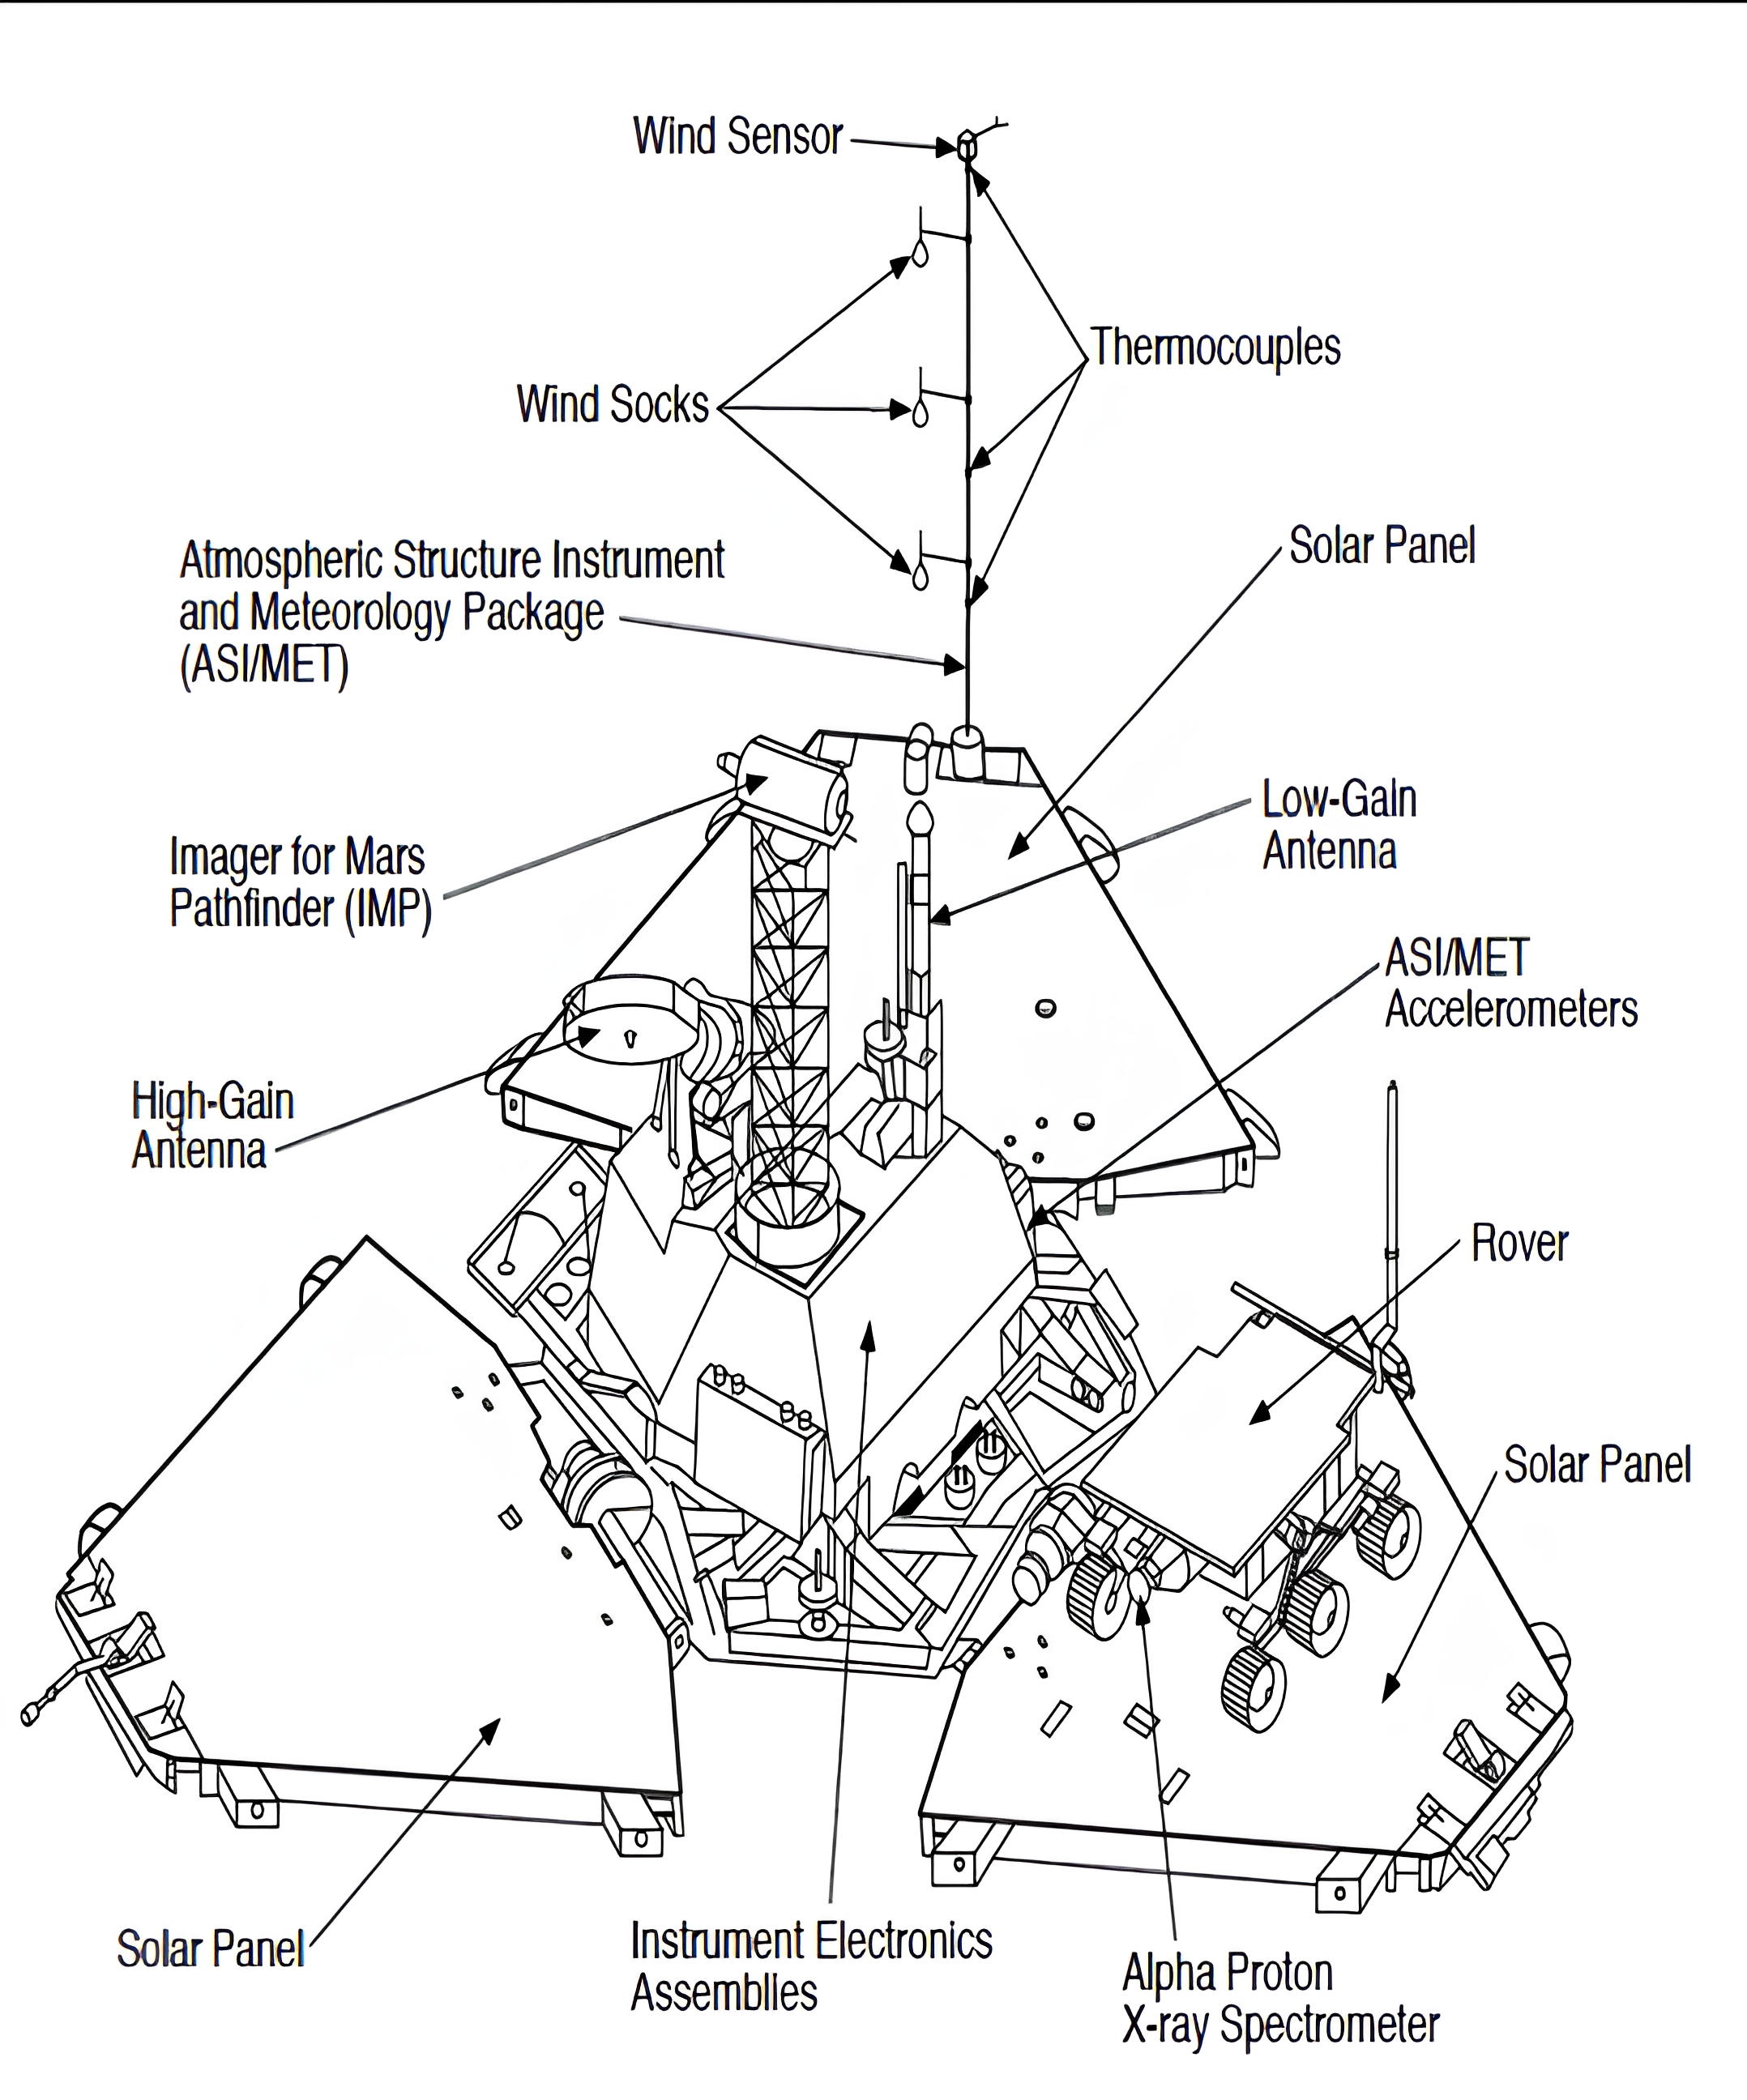
\includegraphics[width=0.7\textwidth]{imagens/mars_pathfinder.png}
\caption{Diagrama da plataforma de pouso da missão Mars Pathfinder da NASA. Repare na câmera rotatória acoplada ao sistema.}
\end{figure}

Ele precisava que a câmera apontasse para placas com letras ao seu redor. Se usasse o alfabeto convencional (26 letras), ele teria que dividir os 360 graus do círculo por 26, o que dá fatias estreitas de cerca de 13,8 graus. A chance de a câmera apontar para a fronteira entre duas letras e gerar ambiguidade era enorme.

A solução? Usar a tabela ASCII (que mapeia texto em números) em formato \textbf{hexadecimal}. Como o hexadecimal possui apenas 16 símbolos (0 a 9 e A a F), ele pôde dividir os 360 graus por 16. O resultado foram fatias largas e seguras de 22,5 graus. Assim, para a Terra enviar a letra "H" (cujo valor na tabela ASCII é 72 em decimal, ou \code{0x48} em hexadecimal), a câmera girava primeiro para a placa \code{4} e depois para a placa \code{8}.

\begin{figure}[H]
\centering
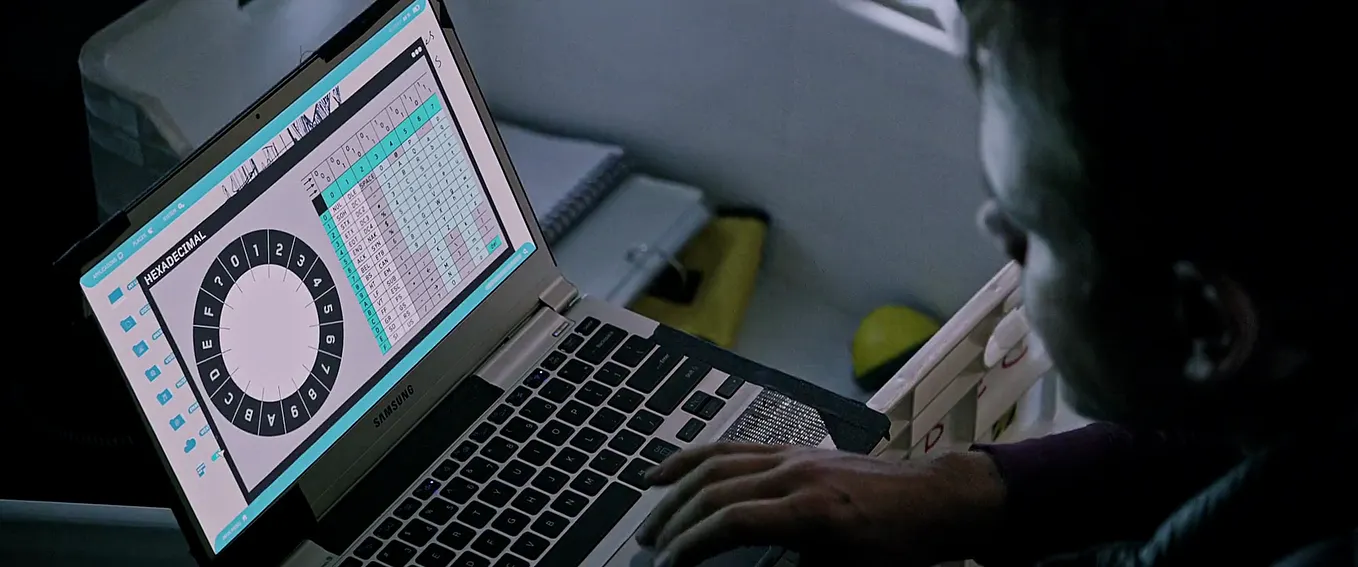
\includegraphics[width=0.8\textwidth]{imagens/mark_watney.png}
\caption{Mark Watney acessando a tabela ASCII pelo notebook de Beth Johanssen.}
\end{figure}

A cena do primeiro contato do filme pode ser vista neste \href{https://www.youtube.com/watch?v=NttUBB98zg4}{link Youtube}.

\section{Memória}

Um programa em execução manipula dados que residem na \textbf{memória} do sistema. Em um computador de propósito geral, essa memória é tipicamente volátil (RAM) e vasta (gigabytes); o sistema operacional gerencia sua alocação de forma praticamente transparente ao programador.

Um microcontrolador como o \ESP{} tem uma realidade bem diferente:

\begin{itemize}
    \item \textbf{Flash} — memória não volátil (mantém os dados sem energia), onde o firmware compilado é gravado. No \ESP{}, tipicamente 4~MB ou mais;
    \item \textbf{SRAM} — memória volátil, rápida, usada para variáveis, pilha (\emph{stack}) e heap durante a execução. No \ESP{}, apenas algumas centenas de kB — ordens de magnitude menor que a RAM de um computador comum.
\end{itemize}

Essa escassez de memória é a razão pela qual, em programação embarcada, escolher o \textbf{tipo de dado} correto para cada variável (assunto do \cref{cap:tipos}) deixa de ser um preciosismo e passa a ser uma decisão de engenharia: usar um \code{int} de 32 bits para armazenar um valor que cabe perfeitamente em 8 bits desperdiça memória que, em um sistema embarcado, pode ser exatamente o que falta.

\section{Pré-processamento}
\label{sec:preprocessamento}

Antes que o compilador propriamente dito veja o código, ele passa por um estágio chamado \textbf{pré-processamento}, controlado por linhas que começam com \code{\#} — as \textbf{diretivas}. Já vimos uma delas, \code{\#include}. Outras diretivas comuns:

\begin{codigoc}{Diretivas de pré-processador}
#include <stdio.h>               // inclui um cabecalho da biblioteca padrao
#include "meu_arquivo.h"         // inclui um cabecalho do proprio projeto

#define PI 3.14159               // define uma macro/constante simbolica
#define QUADRADO(x) ((x) * (x))  // macro com "parametro"

#ifdef DEBUG
    printf("Modo debug ativo\n");
#endif
\end{codigoc}

A diretiva \code{\#define} cria uma \textbf{macro}: onde quer que \code{PI} apareça no código depois dessa linha, o pré-processador o substitui literalmente por \code{3.14159}, \emph{antes} mesmo de o compilador analisar a sintaxe. Diretivas condicionais como \code{\#ifdef}/\code{\#endif} permitem incluir ou excluir trechos inteiros de código dependendo de configurações — um recurso muito usado em projetos embarcados para, por exemplo, ativar mensagens de depuração apenas em builds de desenvolvimento.

Veja como isso se aplica na prática em um código para o ESP32. Podemos criar uma macro chamada \code{DEBUG} e usá-la para "ligar" ou "desligar" o envio de dados pela porta serial:

\begin{codigoc}{Depuração condicional com macros}
#define DEBUG  // Comente esta linha (coloque // na frente) para desativar o debug

void setup() {
    // Inicializa a serial (nao tem problema inicializar mesmo sem usar)
    Serial.begin(115200);

    #ifdef DEBUG
        Serial.println("Sistema iniciado. Modo DEBUG ativo.");
    #endif
}

void loop() {
    int leitura = analogRead(34); // Leitura de um sensor qualquer

    #ifdef DEBUG
        Serial.print("Valor lido pelo sensor: ");
        Serial.println(leitura);
    #endif

    // A logica principal do programa continua aqui, 
    // sem interrupcoes da serial se o DEBUG estiver desativado
    delay(1000);
}
\end{codigoc}

Essa técnica é extremamente poderosa. Ela permite que você encha o seu código de mensagens úteis para investigar o comportamento do sistema durante o desenvolvimento. Quando o projeto estiver pronto para uso real, basta comentar a primeira linha (\code{// \#define DEBUG}). O pré-processador, então, apagará invisivelmente tudo o que estiver entre os blocos \code{\#ifdef DEBUG} e \code{\#endif} antes da compilação. O resultado? Um firmware final menor, mais rápido e que não desperdiça processamento enviando texto para uma porta USB vazia.

\section{Compilação}
\label{sec:compilacao}

O termo ``compilar'' esconde, na verdade, quatro etapas distintas:

\begin{enumerate}
    \item \textbf{Pré-processamento} — expande \code{\#include}, \code{\#define} e diretivas condicionais, produzindo um único arquivo de código-fonte ``puro'';
    \item \textbf{Compilação} — traduz o código C em código assembly equivalente para a arquitetura de destino;
    \item \textbf{Montagem (\emph{assembly})} — converte o código assembly em código de máquina, gerando um arquivo objeto (\code{.o});
    \item \textbf{Ligação (\emph{linking})} — combina o(s) arquivo(s) objeto com as bibliotecas necessárias (como a implementação de \code{printf}) em um único executável.
\end{enumerate}

O \code{gcc} executa essas quatro etapas automaticamente, mas é possível observá-las de forma isolada com a seguir:

\begin{codigobash}{Etapas de compilação separadas}
$ gcc -E hello_world.c -o hello_world.i   # so o pre-processador
$ gcc -S hello_world.i -o hello_world.s   # gera assembly
$ gcc -c hello_world.s -o hello_world.o   # gera arquivo objeto
$ gcc hello_world.o -o hello_world        # linka e gera o executavel
\end{codigobash}

\begin{esp32box}
Ao compilar um projeto para o \ESP{} no PlatformIO, essas mesmas quatro etapas acontecem — só que usando um compilador \textbf{cruzado} (\emph{cross-compiler}): o código roda no seu computador (arquitetura x86/ARM), mas o binário gerado é destinado a um processador \textbf{Xtensa} (a arquitetura do \ESP{}), completamente diferente. O PlatformIO baixa e gerencia essa toolchain de compilação cruzada automaticamente — é uma das razões pelas quais ele simplifica tanto o processo. Detalhes no \cref{cap:platformio}.
\end{esp32box}

\section{Números pseudoaleatórios}

Muitos programas — jogos, simulações, e também firmwares embarcados — precisam de números aparentemente aleatórios. Como um computador é uma máquina determinística, ele não gera aleatoriedade verdadeira a partir do nada: gera números \textbf{pseudoaleatórios}, calculados por uma fórmula a partir de um valor inicial chamado \textbf{semente} (\emph{seed}).

\begin{codigoc}{Gerando números pseudoaleatórios}
#include <stdio.h>
#include <stdlib.h>
#include <time.h>

int main(void) {

    srand(time(NULL));          // inicializa a semente com o tempo atual
    int dado = (rand() % 6) + 1; // numero pseudoaleatorio entre 1 e 6

    printf("Voce tirou: %d\n", dado);
    return 0;
}
\end{codigoc}

A função \code{srand} define a semente do gerador; usar \code{time(NULL)} (o tempo atual em segundos) garante uma semente diferente a cada execução. A função \code{rand()} retorna um valor inteiro pseudoaleatório; o operador \code{\%} (resto da divisão) é usado para restringir o resultado a um intervalo específico — no exemplo, de 1 a 6, como em um dado de tabuleiro.

\begin{atencao}
\code{rand()} \textbf{não} é adequado para fins criptográficos — sua sequência é previsível se a semente for conhecida. Para geração de números aleatórios seguros, bibliotecas específicas de criptografia devem ser usadas.
\end{atencao}

\chapter{Tipos de Variáveis e Operadores}
\label{cap:tipos}

Uma \textbf{variável} é um espaço nomeado na memória usado para armazenar um valor que pode mudar ao longo da execução do programa. Diferente de linguagens como Python, C exige que o \textbf{tipo} de cada variável seja declarado explicitamente (tipagem estática) — é isso que permite ao compilador saber, entre outras coisas, quantos bytes reservar para ela.

\section{Tipos primitivos}

\begin{table}[h]
\centering
\begin{tabular}{@{}lll@{}}
\toprule
\textbf{Tipo} & \textbf{Uso típico} & \textbf{Tamanho comum*} \\
\midrule
\code{char}   & um caractere / inteiro pequeno & 1 byte \\
\code{int}    & número inteiro                 & 4 bytes \\
\code{float}  & número em ponto flutuante (precisão simples) & 4 bytes \\
\code{double} & número em ponto flutuante (precisão dupla)   & 8 bytes \\
\code{bool}\textsuperscript{†} & valor lógico (verdadeiro/falso) & 1 byte \\
\bottomrule
\end{tabular}
\caption{Tipos primitivos da linguagem C. *O tamanho exato depende da arquitetura e do compilador — nunca assuma, use \code{sizeof}. †\code{bool} requer \code{\#include <stdbool.h>}.}
\end{table}

Os tipos \code{int}, \code{char} e \code{double} ainda podem ser modificados por qualificadores:

\begin{codigoc}{Qualificadores de tipo}
short int   a;   // inteiro "curto" (tipicamente 2 bytes)
long int    b;   // inteiro "longo" (tipicamente 4 ou 8 bytes)
long long   c;   // inteiro "bem longo" (tipicamente 8 bytes)

unsigned int d;  // apenas valores nao-negativos (dobra o limite superior)
signed int   e;  // admite valores negativos (comportamento padrao de "int")
\end{codigoc}

Por padrão, os tipos inteiros são \code{signed} (admitem valores negativos, usando uma representação chamada complemento de dois). Adicionar \code{unsigned} descarta o sinal e usa todos os bits para magnitude — um \code{uint8\_t} (8 bits sem sinal) vai de 0 a 255; sua versão com sinal, de $-128$ a $127$.

\begin{codigoc}{Descobrindo o tamanho de um tipo}
#include <stdio.h>

int main(void) {
    printf("sizeof(int)    = %zu bytes\n", sizeof(int));
    printf("sizeof(double) = %zu bytes\n", sizeof(double));
    printf("sizeof(char)   = %zu bytes\n", sizeof(char));
    return 0;
}
\end{codigoc}

O operador \code{sizeof} retorna, em tempo de compilação, o número de bytes ocupados por um tipo ou variável — é a ferramenta certa para nunca precisar ``chutar'' o tamanho de nada.

\begin{atencao}
A linguagem C \textbf{garante apenas tamanhos mínimos} para os tipos primitivos, não tamanhos exatos — \code{int} pode ter 2, 4 ou até 8 bytes dependendo da plataforma e do compilador. Código que assume um tamanho fixo para \code{int} pode compilar perfeitamente em um computador e se comportar de forma diferente (ou quebrar) em um microcontrolador. É exatamente esse problema que a próxima seção resolve.
\end{atencao}

\section{Tipos de largura fixa: \code{stdint.h}}

Para eliminar essa ambiguidade — crítica em sistemas embarcados, onde o tamanho exato de cada variável impacta diretamente no uso de uma memória escassa —, a biblioteca padrão \code{<stdint.h>} define tipos com largura \textbf{garantida}:

\begin{table}[h]
\centering
\begin{tabular}{@{}ll@{}}
\toprule
\textbf{Tipo} & \textbf{Descrição} \\
\midrule
\code{int8\_t}  / \code{uint8\_t}  & inteiro de 8 bits, com/sem sinal (0 a 255) \\
\code{int16\_t} / \code{uint16\_t} & inteiro de 16 bits, com/sem sinal (0 a 65\,535) \\
\code{int32\_t} / \code{uint32\_t} & inteiro de 32 bits, com/sem sinal (0 a $2^{32}\!-\!1$) \\
\code{int64\_t} / \code{uint64\_t} & inteiro de 64 bits, com/sem sinal \\
\bottomrule
\end{tabular}
\caption{Tipos de largura fixa de \code{<stdint.h>}.}
\end{table}

\begin{esp32box}
No código de firmware para o \ESP{} (e em praticamente todo código embarcado sério), \code{uint8\_t}, \code{uint16\_t} e \code{uint32\_t} são usados com muito mais frequência do que \code{int} puro. O motivo é duplo: primeiro, previsibilidade — os registradores dos periféricos do chip exigem tamanhos exatos; segundo, economia de memória — se um valor de sensor nunca ultrapassa 255, guardá-lo em \code{uint8\_t} em vez de \code{int} (que pode ocupar o quádruplo do espaço) é uma escolha consciente de engenharia, não um exagero.
\end{esp32box}

\section{Operadores}

\subsection{Aritméticos}

\begin{table}[h]
\centering
\begin{tabular}{@{}cll@{}}
\toprule
\textbf{Operador} & \textbf{Significado} & \textbf{Exemplo} \\
\midrule
\code{+} & adição               & \code{a + b} \\
\code{-} & subtração            & \code{a - b} \\
\code{*} & multiplicação        & \code{a * b} \\
\code{/} & divisão              & \code{a / b} \\
\code{\%} & resto da divisão (módulo) & \code{a \% b} \\
\bottomrule
\end{tabular}
\caption{Operadores aritméticos.}
\end{table}

\begin{atencao}
A divisão entre dois inteiros em C é sempre \textbf{inteira} — o resultado é truncado, não arredondado. \code{7 / 2} vale \code{3}, não \code{3.5}. Para obter um resultado fracionário, pelo menos um dos operandos precisa ser de ponto flutuante: \code{7.0 / 2} vale \code{3.5}.
\end{atencao}

\subsection{Relacionais e lógicos}

\begin{table}[h]
\centering
\begin{tabular}{@{}cl@{}c@{}cl@{}}
\toprule
\multicolumn{2}{c}{\textbf{Relacionais}} & & \multicolumn{2}{c}{\textbf{Lógicos}} \\
\cmidrule(r){1-2} \cmidrule(l){4-5}
\code{==} & igual a & & \code{\&\&} & E lógico (\emph{and}) \\
\code{!=} & diferente de & & \code{||} & OU lógico (\emph{or}) \\
\code{>} \ \code{<} & maior / menor que & & \code{!} & NÃO lógico (\emph{not}) \\
\code{>=} \ \code{<=} & maior/menor ou igual & & & \\
\bottomrule
\end{tabular}
\caption{Operadores relacionais e lógicos — o resultado é sempre 0 (falso) ou 1 (verdadeiro).}
\end{table}

\begin{atencao}
Um dos erros mais clássicos em C é confundir o operador de \textbf{atribuição} (\code{=}) com o de \textbf{comparação} (\code{==}). A expressão \code{if (x = 5)} é \emph{sintaticamente válida}: ela atribui 5 a \code{x} e depois avalia esse resultado (sempre verdadeiro, pois 5 é diferente de zero) — quase nunca é isso que se pretendia escrever.
\end{atencao}

\subsection{Bit a bit (\emph{bitwise})}

Operadores bit a bit atuam diretamente sobre a representação binária dos operandos, bit por bit — e são especialmente importantes em programação embarcada.

\begin{table}[h]
\centering
\begin{tabular}{@{}cll@{}}
\toprule
\textbf{Operador} & \textbf{Significado} & \textbf{Exemplo} \\
\midrule
\code{\&} & E bit a bit (AND)      & \code{0b1100 \& 0b1010 == 0b1000} \\
\code{|}  & OU bit a bit (OR)      & \code{0b1100 | 0b1010 == 0b1110} \\
\code{\textasciicircum} & OU exclusivo (XOR) & \code{0b1100 \textasciicircum\ 0b1010 == 0b0110} \\
\code{\textasciitilde} & complemento (NOT) & \code{\textasciitilde 0b0000 == 0b1111} \\
\code{<<} & deslocamento à esquerda & \code{1 << 3 == 0b1000} (=8) \\
\code{>>} & deslocamento à direita  & \code{8 >> 2 == 0b0010} (=2) \\
\bottomrule
\end{tabular}
\caption{Operadores bit a bit.}
\end{table}

\begin{esp32box}
Operadores bit a bit são a ferramenta padrão para manipular \textbf{registradores} de periféricos e criar \textbf{máscaras de bits} — muito usadas para representar, de forma compacta, o estado de vários pinos ou dispositivos digitais em uma única variável. Por exemplo, o estado de 8 relés (ligado/desligado) cabe inteiro em um único \code{uint8\_t}, um bit por relé:
\begin{minted}{c}
uint8_t estado_reles = 0;

estado_reles |= (1 << 3);   // liga o rele numero 3
estado_reles &= ~(1 << 5);  // desliga o rele numero 5

if (estado_reles & (1 << 3)) {   // verifica se o rele 3 esta ligado
    printf("Rele 3 esta ligado\n");
}
\end{minted}
O operador \code{<<} desloca o bit \code{1} para a posição correspondente ao dispositivo desejado; \code{|=} liga esse bit sem afetar os demais; \code{\&= \textasciitilde(...)} desliga apenas ele. Voltaremos a essa ideia de forma prática ao ler e escrever pinos digitais no \cref{cap:gpio}.
\end{esp32box}

\subsection{Atribuição composta}

\begin{codigoc}{Operadores de atribuição composta}
int contador = 0;

contador += 5;   // equivalente a: contador = contador + 5;
contador -= 2;   // equivalente a: contador = contador - 2;
contador *= 3;   // equivalente a: contador = contador * 3;
contador /= 2;   // equivalente a: contador = contador / 2;

contador++;      // incrementa em 1 (equivalente a contador += 1)
contador--;      // decrementa em 1 (equivalente a contador -= 1)
\end{codigoc}

\begin{dica}
\code{contador++} (pós-incremento) e \code{++contador} (pré-incremento) têm o mesmo efeito \emph{sobre a variável}, mas diferem no \emph{valor retornado pela expressão} quando usados dentro de outra operação — por exemplo, \code{y = x++} atribui a \code{y} o valor \emph{antigo} de \code{x} e só depois incrementa; \code{y = ++x} incrementa primeiro e atribui o novo valor. Quando o incremento é usado sozinho, em sua própria linha, essa diferença não importa.
\end{dica}

\section{Conversão de tipos (\emph{casting})}

Quando uma expressão mistura tipos diferentes, C converte automaticamente os valores para um tipo comum antes de operar — a chamada \textbf{conversão implícita}. Por exemplo, a operação \code{7.0 / 2} funciona porque o \code{2} (inteiro) é implicitamente convertido para \code{2.0} (ponto flutuante) antes da divisão.

Também é possível forçar uma conversão explicitamente, escrevendo o tipo desejado entre parênteses antes da expressão — o chamado \textbf{cast}:

\begin{codigoc}{Conversão explícita de tipos}
#include <stdio.h>

int main(void) {
    int total = 7, quantidade = 2;

    float media_errada = total / quantidade;          // 3.0 (divisao inteira antes!)
    float media_certa  = (float) total / quantidade;   // 3.5 (cast antes da divisao)

    printf("%.1f\n", media_errada);
    printf("%.1f\n", media_certa);

    return 0;
}
\end{codigoc}

\begin{atencao}
Converter de um tipo ``maior'' para um ``menor'' (por exemplo, \code{double} para \code{int}, ou \code{int} para \code{uint8\_t}) pode \textbf{truncar} ou \textbf{perder informação}: \code{(int) 3.99} vale \code{3}, não \code{4} (a parte fracionária é simplesmente descartada, sem arredondar); atribuir o valor \code{300} a uma variável \code{uint8\_t} (que só representa até 255) produz um resultado \emph{enrolado} (\emph{overflow}), não um erro — o compilador, em geral, nem avisa.
\end{atencao}

\begin{esp32box}
Casts explícitos aparecem com frequência no código de firmware, principalmente ao converter a leitura bruta e inteira de um sensor analógico para uma grandeza física em ponto flutuante. É exatamente o que faremos no \cref{cap:adc}: converter o valor devolvido por \code{analogRead()} (um \code{int} entre 0 e 4095) em uma tensão em volts, algo como \code{(float) leitura / 4095.0f * 3.3f}.
\end{esp32box}

\chapter{Entrada e Saída de Dados}
\label{cap:entrada-saida}

Um programa que não troca informação com o mundo exterior tem utilidade limitada. Nesta seção vemos como C lê dados fornecidos pelo usuário (entrada) e como exibe resultados (saída), usando as funções da biblioteca padrão \code{<stdio.h>}.

\section{Saída formatada: \code{printf}}

Já usamos \code{printf} para exibir texto fixo. Seu verdadeiro poder está nos \textbf{especificadores de formato}, que permitem inserir valores de variáveis dentro da string de saída.

\begin{codigoc}{Especificadores de formato}
#include <stdio.h>

int main(void) {
    int idade = 25;
    float altura = 1.78f;
    char inicial = 'A';

    printf("Idade: %d anos\n", idade);
    printf("Altura: %.2f m\n", altura);
    printf("Inicial: %c\n", inicial);
    printf("Idade em hex: %x, em octal: %o\n", idade, idade);

    return 0;
}
\end{codigoc}

\begin{table}[h]
\centering
\begin{tabular}{@{}ll@{}}
\toprule
\textbf{Especificador} & \textbf{Tipo} \\
\midrule
\code{\%d} / \code{\%i} & inteiro com sinal (\code{int}) \\
\code{\%u}  & inteiro sem sinal (\code{unsigned int}) \\
\code{\%f}  & ponto flutuante (\code{float}/\code{double}) \\
\code{\%c}  & caractere único (\code{char}) \\
\code{\%s}  & string (\code{char *}) \\
\code{\%x} / \code{\%X} & inteiro em hexadecimal (minúsculo/maiúsculo) \\
\code{\%o}  & inteiro em octal \\
\code{\%p}  & endereço de ponteiro \\
\code{\%\%} & imprime o caractere \code{\%} literal \\
\bottomrule
\end{tabular}
\caption{Principais especificadores de formato de \code{printf}/\code{scanf}.}
\end{table}

O especificador pode incluir modificadores de precisão e largura: \code{\%.2f} imprime um ponto flutuante com duas casas decimais; \code{\%5d} reserva um campo de 5 caracteres de largura, alinhado à direita.

\section{Entrada formatada: \code{scanf}}

A função \code{scanf} lê dados digitados pelo usuário no terminal, seguindo a mesma lógica de especificadores de \code{printf} — porém exige o \textbf{endereço} da variável onde o valor lido será armazenado, indicado pelo operador \code{\&} (introduzido formalmente no \cref{cap:ponteiros}).

\begin{codigoc}{Lendo dados do teclado}
#include <stdio.h>

int main(void) {
    int idade;

    printf("Digite sua idade: ");
    scanf("%d", &idade);

    printf("Voce tem %d anos.\n", idade);
    return 0;
}
\end{codigoc}

\begin{atencao}
Esquecer o \code{\&} antes da variável em \code{scanf} é um erro comum e perigoso: em vez do endereço da variável, \code{scanf} recebe o \emph{valor} nela contido, interpretado como se fosse um endereço de memória — e tenta escrever ali. O compilador frequentemente emite um aviso (\emph{warning}), mas o programa pode compilar mesmo assim e falhar (ou pior, corromper memória) apenas durante a execução.
\end{atencao}

\begin{dica}
\code{scanf} é útil para aprender, mas tem limitações importantes de segurança e de tratamento de erros (não valida corretamente o que foi digitado, e é fácil causar \emph{buffer overflow} ao ler strings sem limitar o tamanho). Em código de produção, funções como \code{fgets} combinada com \code{sscanf} costumam ser preferidas.
\end{dica}

\section{Caracteres e strings}

Uma \code{string} em C não é um tipo primitivo — é, na prática, um vetor de caracteres (\code{char[]}) terminado por um caractere nulo especial, \code{'\textbackslash 0'}, que marca seu fim. Esse assunto será retomado com mais profundidade no \cref{cap:arranjos}.

\begin{codigoc}{Strings como vetores de caracteres}
#include <stdio.h>

int main(void) {
    char nome[20];

    printf("Digite seu nome: ");
    scanf("%19s", nome);   // le ate 19 caracteres (+ '\0' automatico)

    printf("Ola, %s!\n", nome);
    return 0;
}
\end{codigoc}

\section{Sequências de escape}

Dentro de strings e caracteres literais, a barra invertida introduz caracteres especiais que não têm representação visual direta:

\begin{table}[h]
\centering
\begin{tabular}{@{}ll@{}}
\toprule
\textbf{Sequência} & \textbf{Significado} \\
\midrule
\code{\textbackslash n} & nova linha (\emph{newline}) \\
\code{\textbackslash t} & tabulação horizontal \\
\code{\textbackslash r} & retorno de carro (\emph{carriage return}) \\
\code{\textbackslash 0} & caractere nulo (fim de string) \\
\code{\textbackslash \textbackslash} & barra invertida literal \\
\code{\textbackslash "} & aspas duplas literais (dentro de uma string) \\
\bottomrule
\end{tabular}
\caption{Sequências de escape mais comuns.}
\end{table}

\section{Manipulação de arquivos}

A biblioteca \code{<stdio.h>} também fornece funções para ler e escrever arquivos em disco, usando um ponteiro do tipo \code{FILE *} como identificador do arquivo aberto.

\begin{codigoc}{Escrevendo e lendo um arquivo de texto}
#include <stdio.h>

int main(void) {
    FILE *arquivo = fopen("dados.txt", "w");
    if (arquivo == NULL) {
        printf("Erro ao abrir o arquivo!\n");
        return 1;
    }

    fprintf(arquivo, "Temperatura: %d C\n", 27);
    fclose(arquivo);

    return 0;
}
\end{codigoc}

O padrão \code{"w"} abre o arquivo para escrita (criando-o se não existir, ou apagando seu conteúdo se existir); \code{"r"} abre para leitura; \code{"a"} adiciona conteúdo ao final de um arquivo existente. Verificar se \code{fopen} retornou \code{NULL} é essencial — é assim que a função sinaliza falha (por exemplo, permissão negada ou disco cheio).

\section{Saída como ferramenta de depuração}
\label{sec:printf-debug}

Além de comunicar resultados ao usuário final, a saída de um programa é, na prática, a ferramenta de \textbf{depuração} (\emph{debug}) mais usada por programadores iniciantes e experientes — imprimir o valor de uma variável em pontos estratégicos do código para entender \emph{por que} ele não está se comportando como esperado é uma técnica tão comum que tem até um apelido: \emph{print debugging}.

\begin{codigoc}{Depurando um cálculo com printf}
#include <stdio.h>

int main(void) {
    int total = 0;

    for (int i = 1; i <= 5; i++) {
        total += i;
        printf("[DEBUG] i = %d, total acumulado = %d\n", i, total);
    }

    printf("Resultado final: %d\n", total);
    return 0;
}
\end{codigoc}

\begin{dica}
Um prefixo consistente, como \code{[DEBUG]} no exemplo acima, ajuda a distinguir mensagens de depuração (que normalmente serão removidas ou desativadas depois) das mensagens de saída ``de verdade'' do programa. Ferramentas de depuração mais sofisticadas (como o \emph{debugger} \code{gdb}, capaz de pausar a execução e inspecionar variáveis sem precisar de nenhum \code{printf}) existem e são valiosas, mas a técnica de espalhar mensagens de saída pelo código continua sendo, de longe, a mais rápida e mais usada no dia a dia — especialmente em sistemas embarcados, como veremos a seguir.
\end{dica}

\begin{esp32box}
O \ESP{} não tem, por padrão, teclado nem tela — mas tem algo funcionalmente equivalente: a \textbf{porta serial} (UART), conectada ao computador via USB. No framework Arduino, a saída não passa pelo \code{printf} da biblioteca padrão diretamente: usa-se o objeto \code{Serial}, inicializado uma única vez em \code{setup()} com \code{Serial.begin(115200);}. A partir daí, \code{Serial.println("mensagem")} exibe uma linha de texto, e \code{Serial.printf("valor: \%d\textbackslash n", x)} aceita exatamente os \textbf{mesmos especificadores de formato} de \code{printf} apresentados neste capítulo — o conhecimento é diretamente reaproveitável, só muda a forma de chamar a função. É assim que toda a técnica de depuração por mensagens de saída, vista acima, se transporta para o firmware: em vez de rodar em um terminal, as mensagens \code{[DEBUG]} aparecem no \textbf{monitor serial} do PlatformIO. O \cref{cap:serial} é dedicado inteiramente a essa prática no \ESP{}.

Já \code{scanf} praticamente não tem uso em firmware embarcado — a ``entrada'' normalmente vem de sensores e botões, não de um teclado, como veremos a partir do \cref{cap:gpio}.

Quanto a arquivos: o \ESP{} pode montar um sistema de arquivos dentro da própria memória flash (usando bibliotecas como LittleFS, também disponíveis no framework Arduino), permitindo abrir, ler e escrever arquivos com uma API muito parecida com a de \code{<stdio.h>} — extremamente útil para salvar configurações ou registros que precisam sobreviver a um desligamento.
\end{esp32box}

\chapter{Estruturas de Decisão}
\label{cap:decisao}

Até aqui, todo código apresentado executa suas instruções sequencialmente, uma após a outra, do início ao fim. Estruturas de decisão permitem que o programa escolha \emph{qual} caminho seguir, dependendo de uma condição — é isso que dá a um programa a capacidade de reagir de forma diferente a diferentes situações.

\section{\code{if} / \code{else}}

\begin{codigoc}{Estrutura if / else if / else}
#include <stdio.h>

int main(void) {
    int temperatura = 32;

    if (temperatura > 30) {
        printf("Esta quente!\n");
    } else if (temperatura < 15) {
        printf("Esta frio!\n");
    } else {
        printf("Temperatura agradavel.\n");
    }

    return 0;
}
\end{codigoc}

Em C, \textbf{qualquer valor diferente de zero é considerado verdadeiro}; apenas o valor \code{0} é considerado falso. Isso significa que \code{if (10)} sempre executa seu bloco, e \code{if (0)} nunca executa — mesmo sem envolver nenhum operador relacional explícito.

\begin{dica}
Quando o bloco de um \code{if} (ou de qualquer estrutura de controle) contém uma única instrução, as chaves são opcionais. Ainda assim, é considerada boa prática sempre usá-las — isso evita um erro clássico onde uma segunda linha, adicionada depois por engano fora das chaves, passa a ser executada incondicionalmente.
\end{dica}

\section{Operador ternário}

Para condicionais simples que retornam um valor, C oferece uma forma compacta:

\begin{codigoc}{Operador ternário}
int a = 10, b = 20;
int maior = (a > b) ? a : b;   // "se a > b, entao a, senao b"

printf("O maior valor e %d\n", maior);
\end{codigoc}

\section{\code{switch}}

Quando uma mesma variável precisa ser comparada contra vários valores possíveis, o \code{switch} costuma ser mais legível do que uma longa cadeia de \code{else if}:

\begin{codigoc}{Estrutura switch}
#include <stdio.h>

int main(void) {
    int dia = 3;

    switch (dia) {
        case 1:
            printf("Segunda-feira\n");
            break;
        case 2:
            printf("Terca-feira\n");
            break;
        case 3:
            printf("Quarta-feira\n");
            break;
        default:
            printf("Dia invalido\n");
    }

    return 0;
}
\end{codigoc}

\begin{atencao}
Esquecer o \code{break} ao final de um \code{case} faz a execução ``cair'' (\emph{fall-through}) para o próximo \code{case}, executando-o também — mesmo que sua condição não tenha sido satisfeita. Às vezes esse comportamento é usado intencionalmente (para agrupar vários casos com a mesma ação), mas na grande maioria das vezes é um bug. O \code{default}, por convenção o último caso, captura qualquer valor não tratado pelos \code{case}s anteriores.
\end{atencao}

\begin{esp32box}
Estruturas \code{switch} são extremamente comuns em firmware para implementar \textbf{máquinas de estado} — por exemplo, controlar as diferentes fases de operação de um dispositivo (``aguardando'', ``conectando ao Wi-Fi'', ``lendo sensor'', ``enviando dados'', ``erro''), onde cada estado é representado por um valor de um \code{enum} (\cref{cap:structs}) e o \code{switch} decide o que fazer em cada um deles a cada iteração do laço principal do programa.
\end{esp32box}

\chapter{Laços de Repetição e Desvios}
\label{cap:repeticao}

Laços (ou \emph{loops}) permitem repetir um bloco de instruções múltiplas vezes, sem precisar reescrevê-lo. C oferece três estruturas de repetição — \code{for}, \code{while} e \code{do-while} — cada uma mais adequada a um cenário específico.

\section{\code{for}}

O laço \code{for} é ideal quando o número de repetições é conhecido (ou calculável) de antemão.

\begin{codigoc}{Laço for}
#include <stdio.h>

int main(void) {
    for (int i = 0; i < 5; i++) {
        printf("Iteracao %d\n", i);
    }
    return 0;
}
\end{codigoc}

A estrutura \code{for (inicialização; condição; incremento)} tem três partes, todas opcionais:

\begin{itemize}
    \item \textbf{Inicialização} — executada uma única vez, antes da primeira iteração (tipicamente declara e inicializa a variável de controle);
    \item \textbf{Condição} — testada \emph{antes} de cada iteração; o laço continua enquanto ela for verdadeira;
    \item \textbf{Incremento} — executado ao final de cada iteração, antes de testar a condição novamente.
\end{itemize}

\section{\code{while}}

O laço \code{while} repete um bloco \emph{enquanto} uma condição permanecer verdadeira, testada sempre no início de cada iteração — inclusive antes da primeira. É a estrutura certa quando o número de repetições não é conhecido de antemão.

\begin{codigoc}{Laço while}
#include <stdio.h>

int main(void) {
    int contador = 5;

    while (contador > 0) {
        printf("Contagem: %d\n", contador);
        contador--;
    }
    printf("Fim!\n");

    return 0;
}
\end{codigoc}

\section{\code{do-while}}

O laço \code{do-while} é semelhante ao \code{while}, mas testa a condição \emph{depois} de cada iteração — garantindo que o bloco execute \textbf{ao menos uma vez}, mesmo que a condição já comece falsa. Isso o torna a estrutura natural para validação de entrada, onde é preciso pedir o dado ao menos uma vez antes de poder avaliar se ele é válido:

\begin{codigoc}{Laço do-while}
#include <stdio.h>

int main(void) {
    int senha, tentativas = 0;

    do {
        printf("Digite a senha: ");
        scanf("%d", &senha);
        tentativas++;
    } while (senha != 1234 && tentativas < 3);

    if (senha == 1234) {
        printf("Acesso liberado!\n");
    } else {
        printf("Numero de tentativas excedido.\n");
    }

    return 0;
}
\end{codigoc}

\begin{esp32box}
Todo firmware embarcado gira, conceitualmente, em torno de um \textbf{laço principal infinito} — algo como \code{while (1) \{ ... \}}, que nunca termina enquanto o dispositivo estiver ligado, lendo sensores e atualizando saídas indefinidamente. No framework Arduino, como veremos no \cref{cap:anatomia}, esse laço já vem pronto: em vez de escrevê-lo você mesmo, basta colocar o código a repetir dentro de uma função chamada \code{loop()} — o próprio framework se encarrega de chamá-la repetidamente, para sempre, por trás dos panos.
\end{esp32box}

\section{\code{break} e \code{continue}}

Dois comandos permitem alterar o fluxo normal de um laço:

\begin{itemize}
    \item \code{break} — interrompe o laço imediatamente, saindo dele por completo;
    \item \code{continue} — pula o restante da iteração atual e avança direto para a próxima.
\end{itemize}

\begin{codigoc}{break e continue}
#include <stdio.h>

int main(void) {
    for (int i = 1; i <= 10; i++) {

        if (i % 2 == 0) {
            continue;   // pula os numeros pares
        }

        if (i > 7) {
            break;      // interrompe o laco ao passar de 7
        }

        printf("%d\n", i);  // imprime: 1, 3, 5, 7
    }
    return 0;
}
\end{codigoc}

\chapter{Funções e Protótipos}
\label{cap:funcoes}

Uma \textbf{função} é um bloco de código nomeado, reutilizável, que realiza uma tarefa específica. Já usamos várias — \code{printf}, \code{scanf}, \code{main} — mas até agora sempre prontas, fornecidas por bibliotecas. Esta seção mostra como criar as suas próprias.

\section{Declarando e chamando funções}

\begin{codigoc}{Uma função simples}
#include <stdio.h>

int soma(int a, int b) {
    int resultado = a + b;
    return resultado;
}

int main(void) {
    int total = soma(5, 3);
    printf("A soma e %d\n", total);
    return 0;
}
\end{codigoc}

Uma definição de função tem quatro partes:

\begin{itemize}
    \item \textbf{Tipo de retorno} (\code{int}) — o tipo do valor devolvido por \code{return}. Use \code{void} quando a função não retorna nenhum valor;
    \item \textbf{Nome} (\code{soma}) — usado para chamá-la em outros pontos do código;
    \item \textbf{Parâmetros} (\code{int a, int b}) — as variáveis que a função recebe como entrada, entre parênteses;
    \item \textbf{Corpo} — o bloco de instruções entre chaves, executado a cada chamada.
\end{itemize}

\section{Passagem de parâmetros por valor}

Em C, argumentos são passados para funções \textbf{por valor}: a função recebe uma \emph{cópia} do dado, não o dado original. Alterações feitas dentro da função não afetam a variável usada na chamada.

\begin{codigoc}{Passagem por valor}
#include <stdio.h>

void dobrar(int x) {
    x = x * 2;   // altera apenas a copia local
}

int main(void) {
    int numero = 10;
    dobrar(numero);
    printf("%d\n", numero);   // ainda imprime 10!
    return 0;
}
\end{codigoc}

Para que uma função possa modificar uma variável do código que a chamou, é preciso passar seu \textbf{endereço} (um ponteiro) em vez do valor — técnica detalhada no \cref{cap:ponteiros}.

\section{Protótipos de funções}

Em C, uma função precisa ser \textbf{conhecida} pelo compilador antes de ser usada. Quando a definição completa de uma função vem depois do ponto onde ela é chamada (ou está em outro arquivo), é preciso declarar um \textbf{protótipo}: a assinatura da função, sem o corpo, terminada em ponto e vírgula.

\begin{codigoc}{Protótipo declarado antes do uso}
#include <stdio.h>

int soma(int a, int b);   // prototipo

int main(void) {
    printf("%d\n", soma(4, 6));  // ja pode ser chamada aqui
    return 0;
}

int soma(int a, int b) {   // definicao completa, depois do uso
    return a + b;
}
\end{codigoc}

\begin{dica}
Protótipos são a razão de existir dos arquivos de cabeçalho (\code{.h}): eles reúnem as assinaturas das funções de um módulo, permitindo que outros arquivos \code{.c} as usem sem precisar ver (ou recompilar) sua implementação completa. Esse padrão é explorado a fundo no \cref{cap:modularizacao}.
\end{dica}

\section{Escopo de variáveis}

O \textbf{escopo} de uma variável é a região do código onde ela existe e pode ser acessada. Variáveis declaradas dentro de uma função (ou de qualquer bloco \code{\{ \}}) são \textbf{locais} — existem apenas enquanto aquele bloco está em execução, e são invisíveis fora dele. Variáveis declaradas fora de qualquer função são \textbf{globais} — visíveis (e modificáveis) por todas as funções do arquivo.

\begin{codigoc}{Escopo local vs. global}
#include <stdio.h>

int contador_global = 0;   // variavel global

void incrementar(void) {
    int passo = 1;          // variavel local a "incrementar"
    contador_global += passo;
}

int main(void) {
    incrementar();
    incrementar();
    printf("%d\n", contador_global);   // imprime 2
    // printf("%d\n", passo);          // ERRO: "passo" nao existe aqui
    return 0;
}
\end{codigoc}

\begin{atencao}
Variáveis globais são convenientes, mas usadas em excesso tornam o código difícil de entender e depurar — qualquer função pode alterá-las a qualquer momento, criando dependências ocultas. Prefira sempre passar dados explicitamente por parâmetros e devolvê-los por \code{return} quando possível.
\end{atencao}

\subsection{Variáveis locais \code{static}}

Uma variável local declarada com o qualificador \code{static} tem um comportamento híbrido: continua visível apenas dentro da função onde foi declarada (como qualquer variável local), mas seu valor \textbf{persiste entre chamadas} — em vez de ser recriada do zero a cada chamada da função, ela é inicializada uma única vez, na primeira execução, e mantém seu valor de uma chamada para a próxima.

\begin{codigoc}{Uma variável static mantém seu valor entre chamadas}
#include <stdio.h>

void contar_chamadas(void) {
    static int chamadas = 0;   // inicializada uma unica vez
    chamadas++;
    printf("Esta funcao ja foi chamada %d vez(es)\n", chamadas);
}

int main(void) {
    contar_chamadas();   // "1 vez(es)"
    contar_chamadas();   // "2 vez(es)"
    contar_chamadas();   // "3 vez(es)"
    return 0;
}
\end{codigoc}

Isso é útil sempre que uma função precisa ``lembrar'' algo de sua execução anterior — um contador de eventos, o último valor processado — sem recorrer a uma variável global.

\begin{esp32box}
Em firmware embarcado, algumas variáveis globais são difíceis de evitar por completo — por exemplo, uma variável compartilhada entre a rotina principal e uma \textbf{interrupção} (\cref{cap:interrupcoes}), que roda de forma assíncrona e precisa sinalizar eventos para o resto do programa. Nesses casos, a variável costuma ser declarada com o qualificador \code{volatile}, que instrui o compilador a nunca otimizar (ou assumir como constante) o acesso àquela variável — porque seu valor pode mudar a qualquer momento, fora do fluxo normal do código.
\end{esp32box}

\chapter{Arranjos: Vetores}
\label{cap:arranjos}

Um \textbf{arranjo} (\emph{array}), ou \textbf{vetor}, é uma coleção de elementos do mesmo tipo, armazenados em posições de memória contíguas e acessados por um índice numérico. É a estrutura de dados mais fundamental para trabalhar com múltiplos valores relacionados — uma lista de leituras de sensor, o histórico de temperaturas de um dia, as últimas N amostras de um sinal.

\section{Declarando e percorrendo um vetor}

\begin{codigoc}{Declarando e usando um vetor}
#include <stdio.h>

int main(void) {
    int temperaturas[5] = {21, 23, 19, 25, 22};

    for (int i = 0; i < 5; i++) {
        printf("Dia %d: %d C\n", i, temperaturas[i]);
    }

    return 0;
}
\end{codigoc}

Pontos essenciais sobre vetores em C:

\begin{itemize}
    \item \textbf{Índices começam em 0} — o primeiro elemento de \code{temperaturas} é \code{temperaturas[0]}, e o último, em um vetor de 5 elementos, é \code{temperaturas[4]};
    \item O \textbf{tamanho é fixo} após a declaração — um vetor declarado com 5 posições sempre ocupará espaço para 5 elementos; não é possível ``crescer'' um vetor comum em tempo de execução (para isso, veja alocação dinâmica no \cref{cap:ponteiros});
    \item C \textbf{não verifica limites automaticamente}: acessar \code{temperaturas[10]} em um vetor de 5 posições não gera um erro imediato — apenas lê (ou escreve) memória fora da área reservada, um comportamento indefinido e uma fonte clássica de bugs graves.
\end{itemize}

\begin{atencao}
Esse tipo de acesso fora dos limites (\emph{buffer overflow}) é uma das causas mais comuns de falhas de segurança em software escrito em C. Sempre garanta, por construção do seu código, que o índice usado está dentro do intervalo válido do vetor.
\end{atencao}

\section{Vetores e strings}

Como visto no \cref{cap:entrada-saida}, uma string em C é simplesmente um vetor de \code{char} terminado pelo caractere nulo \code{'\textbackslash 0'}:

\begin{codigoc}{Uma string é um vetor de char}
#include <stdio.h>

int main(void) {
    char saudacao[6] = {'H', 'e', 'l', 'l', 'o', '\0'};
    // equivalente, e muito mais pratico, a:
    char saudacao2[] = "Hello";

    printf("%s\n", saudacao2);
    return 0;
}
\end{codigoc}

\section{Passando arranjos para funções}

Quando um vetor é passado como argumento para uma função, o que de fato é passado é um \textbf{ponteiro} para seu primeiro elemento — não uma cópia de todos os seus dados. Por isso, é comum (e necessário) passar também o tamanho do vetor como um parâmetro separado, já que a função não tem como saber onde ele termina apenas olhando para o ponteiro.

\begin{codigoc}{Vetor como parâmetro de função}
#include <stdio.h>

float media(int vetor[], int tamanho) {
    int soma = 0;
    for (int i = 0; i < tamanho; i++) {
        soma += vetor[i];
    }
    return (float) soma / tamanho;
}

int main(void) {
    int leituras[4] = {30, 32, 28, 31};
    printf("Media: %.1f\n", media(leituras, 4));
    return 0;
}
\end{codigoc}

\begin{esp32box}
Vetores são onipresentes em firmware embarcado: um buffer para armazenar bytes recebidos pela porta serial, uma tabela de valores de calibração de um sensor, ou um histórico circular das últimas N leituras de temperatura para calcular uma média móvel. Como a memória RAM do \ESP{} é limitada, o \textbf{tamanho} desses vetores costuma ser dimensionado com muito mais cuidado do que em um programa de computador — reservar um vetor de 10.000 posições ``só por garantia'' pode facilmente esgotar a memória disponível do chip.
\end{esp32box}

\chapter{Ponteiros e Alocação Dinâmica de Memória}
\label{cap:ponteiros}

Ponteiros são, ao mesmo tempo, o recurso mais poderoso e o mais temido por quem está aprendendo C. Eles são também o motivo pelo qual C permanece tão relevante em programação de baixo nível: nenhuma outra construção da linguagem dá ao programador controle tão direto sobre a memória do computador.

\section{O que é um ponteiro}

Toda variável, ao ser declarada, ocupa um espaço na memória identificado por um \textbf{endereço}. Um \textbf{ponteiro} é uma variável cujo valor \emph{é} o endereço de outra variável — em vez de armazenar um dado diretamente, ele aponta para onde esse dado está guardado.

\begin{codigoc}{Endereços e ponteiros}
#include <stdio.h>

int main(void) {
    int idade = 25;
    int *ptr_idade = &idade;   // ptr_idade guarda o ENDERECO de idade

    printf("Valor de idade:        %d\n", idade);
    printf("Endereco de idade:     %p\n", (void *) &idade);
    printf("Valor de ptr_idade:    %p\n", (void *) ptr_idade);
    printf("Valor apontado por ptr: %d\n", *ptr_idade);

    return 0;
}
\end{codigoc}

Dois operadores são essenciais para trabalhar com ponteiros:

\begin{itemize}
    \item \code{\&} (\emph{address-of}) — obtém o endereço de uma variável: \code{\&idade};
    \item \code{*} (\emph{dereference}, ou ``desreferenciação'') — acessa o valor armazenado no endereço apontado: \code{*ptr\_idade}.
\end{itemize}

\begin{nota}
O mesmo símbolo \code{*} tem dois papéis diferentes dependendo do contexto: na \textbf{declaração} (\code{int *ptr}), ele indica que a variável é um ponteiro; em uma \textbf{expressão} (\code{*ptr = 10}), ele desreferencia o ponteiro, acessando o valor apontado.
\end{nota}

\section{Ponteiros como parâmetros de função}

Como vimos no \cref{cap:funcoes}, argumentos são passados por valor em C — uma função não pode alterar diretamente uma variável do código que a chamou. Ponteiros resolvem exatamente esse problema: em vez de passar o valor, passa-se o \emph{endereço}, permitindo que a função modifique o dado original.

\begin{codigoc}{Modificando uma variável via ponteiro}
#include <stdio.h>

void dobrar(int *x) {
    *x = *x * 2;   // modifica o valor no endereco apontado
}

int main(void) {
    int numero = 10;
    dobrar(&numero);
    printf("%d\n", numero);   // agora imprime 20
    return 0;
}
\end{codigoc}

\begin{dica}
É exatamente por esse mecanismo que \code{scanf("\%d", \&idade)} funciona: sem o \code{\&}, a função receberia apenas uma cópia do valor de \code{idade} e não teria como escrever o dado lido de volta na variável original.
\end{dica}

\section{Ponteiros e vetores}

O nome de um vetor, usado sozinho em uma expressão, é convertido automaticamente para um ponteiro ao seu primeiro elemento — é por isso que, no \cref{cap:arranjos}, passar um vetor para uma função na prática passa um ponteiro.

\begin{codigoc}{Aritmética de ponteiros}
#include <stdio.h>

int main(void) {
    int valores[4] = {10, 20, 30, 40};
    int *p = valores;   // p aponta para valores[0]

    printf("%d\n", *p);        // 10
    printf("%d\n", *(p + 1));  // 20  (equivalente a valores[1])
    printf("%d\n", *(p + 2));  // 30  (equivalente a valores[2])

    return 0;
}
\end{codigoc}

Somar 1 a um ponteiro não avança um único byte — avança o \textbf{tamanho do tipo apontado}. Em \code{int *p}, \code{p + 1} avança 4 bytes (o tamanho de um \code{int}), apontando corretamente para o próximo elemento do vetor.

\section{Alocação dinâmica de memória}

Todas as variáveis vistas até agora têm tamanho fixo, decidido em tempo de compilação, e residem na \textbf{pilha} (\emph{stack}) — uma região de memória gerenciada automaticamente. Às vezes, porém, o tamanho necessário só é conhecido em tempo de execução (por exemplo, depende de uma entrada do usuário). Para esses casos, C permite reservar memória manualmente, em uma região chamada \textbf{heap}, usando funções da biblioteca \code{<stdlib.h>}.

\begin{table}[h]
\centering
\begin{tabular}{@{}ll@{}}
\toprule
\textbf{Função} & \textbf{Finalidade} \\
\midrule
\code{malloc(tamanho)}          & aloca \code{tamanho} bytes, sem inicializar \\
\code{calloc(n, tamanho)}       & aloca \code{n} blocos de \code{tamanho} bytes, zerados \\
\code{realloc(ptr, novo\_tam)}  & redimensiona um bloco previamente alocado \\
\code{free(ptr)}                & libera a memória apontada por \code{ptr} \\
\bottomrule
\end{tabular}
\caption{Funções de alocação dinâmica de \code{<stdlib.h>}.}
\end{table}

\begin{codigoc}{Alocando um vetor em tempo de execução}
#include <stdio.h>
#include <stdlib.h>

int main(void) {
    int n;
    printf("Quantos numeros deseja armazenar? ");
    scanf("%d", &n);

    int *vetor = (int *) malloc(n * sizeof(int));
    if (vetor == NULL) {
        printf("Falha ao alocar memoria!\n");
        return 1;
    }

    for (int i = 0; i < n; i++) {
        vetor[i] = i * i;
        printf("%d ", vetor[i]);
    }
    printf("\n");

    free(vetor);   // devolve a memoria ao sistema
    return 0;
}
\end{codigoc}

\begin{atencao}
Toda chamada a \code{malloc} (ou \code{calloc}/\code{realloc}) bem-sucedida deve ter, mais cedo ou mais tarde, uma chamada correspondente a \code{free}. Esquecer de liberar memória alocada causa \textbf{vazamento de memória} (\emph{memory leak}) — o programa consome cada vez mais memória ao longo do tempo, até eventualmente esgotá-la. Usar um ponteiro \emph{depois} de liberá-lo (um \emph{dangling pointer}) ou liberá-lo duas vezes são igualmente perigosos, e podem causar comportamento indefinido ou travamentos difíceis de depurar.
\end{atencao}

\begin{esp32box}
O \ESP{} tem apenas algumas centenas de kB de RAM disponíveis, compartilhados entre o programa, a pilha e o heap — e, diferente de um computador, não existe memória virtual em disco para ``salvar'' o sistema quando a memória se esgota: se um \code{malloc} falhar por falta de espaço, ele retorna \code{NULL}, e um firmware mal escrito que não verifica isso pode travar ou reiniciar sozinho (um \emph{crash}). Por essa razão, boa parte do código embarcado profissional evita alocação dinâmica sempre que possível, preferindo vetores de tamanho fixo, definidos em tempo de compilação — sacrificando um pouco de flexibilidade em troca de comportamento previsível, essencial em sistemas que muitas vezes precisam funcionar ininterruptamente por meses.
\end{esp32box}

\chapter{Structs e Enumerações}
\label{cap:structs}

Até aqui, cada variável guardava um único valor de um único tipo. Esta seção apresenta ferramentas para agrupar dados relacionados em uma única unidade — essencial para modelar informações do mundo real, como a leitura de um sensor (valor, unidade, instante da medição) ou a configuração de um periférico.

\section{Registros e \code{structs}}

Uma \code{struct} agrupa múltiplas variáveis, de tipos possivelmente diferentes, sob um único nome — cada uma acessível por um \textbf{campo} (\emph{field}).

\begin{codigoc}{Definindo e usando uma struct}
#include <stdio.h>

typedef struct {
    char nome[20];
    float temperatura;
    int  umidade;
} Leitura;

int main(void) {
    Leitura sala = {"Sala de estar", 23.5f, 60};

    printf("%s: %.1f C, %d%% umidade\n",
           sala.nome, sala.temperatura, sala.umidade);

    sala.temperatura = 24.0f;   // acessando e alterando um campo
    return 0;
}
\end{codigoc}

O \code{typedef} antes de \code{struct} cria um \textbf{apelido de tipo}: em vez de escrever \code{struct Leitura sala;} toda vez, basta \code{Leitura sala;}. Campos são acessados com o operador ponto (\code{.}).

\subsection{Structs e ponteiros}

Quando se tem um \textbf{ponteiro} para uma struct (comum ao passá-la para funções, evitando copiar todos os seus campos), o acesso aos campos usa o operador seta (\code{->}) em vez do ponto:

\begin{codigoc}{Acessando campos via ponteiro}
#include <stdio.h>

typedef struct {
    float temperatura;
    int umidade;
} Leitura;

void exibir(Leitura *l) {
    printf("%.1f C, %d%%\n", l->temperatura, l->umidade);
    // equivalente a: (*l).temperatura, (*l).umidade
}

int main(void) {
    Leitura sala = {23.5f, 60};
    exibir(&sala);
    return 0;
}
\end{codigoc}

\section{Enumerações (\code{enum})}

Uma \code{enum} define um conjunto nomeado de constantes inteiras, tornando o código mais legível do que usar números ``mágicos'' soltos pelo texto.

\begin{codigoc}{Definindo uma enumeração}
#include <stdio.h>

typedef enum {
    ESTADO_AGUARDANDO,   // vale 0
    ESTADO_CONECTANDO,   // vale 1
    ESTADO_ATIVO,        // vale 2
    ESTADO_ERRO          // vale 3
} EstadoSistema;

int main(void) {
    EstadoSistema estado = ESTADO_CONECTANDO;

    if (estado == ESTADO_CONECTANDO) {
        printf("Conectando...\n");
    }

    return 0;
}
\end{codigoc}

Por padrão, o primeiro valor de uma \code{enum} vale 0, e cada valor seguinte é o anterior mais 1 — mas isso pode ser sobrescrito explicitamente (\code{ESTADO\_ERRO = 100}, por exemplo). Combinada com um \code{switch} (\cref{cap:decisao}), uma \code{enum} é a base clássica para implementar máquinas de estado em C.

\begin{esp32box}
\code{structs} e \code{enums} são ferramentas centrais para organizar o estado de um projeto de IoT. Uma \code{struct} agrupa naturalmente tudo o que pertence a uma mesma leitura de sensor — valor, unidade, instante da medição —, em vez de espalhar essa informação em várias variáveis soltas; uma \code{enum} representa, de forma legível, os diferentes \textbf{modos de operação} de um dispositivo (por exemplo, \code{MODO\_NORMAL}, \code{MODO\_ALERTA}, \code{MODO\_ECONOMIA}), testados com um \code{switch} a cada iteração do \code{loop()}. Usaremos exatamente essa combinação no projeto integrador do \cref{cap:projeto-final}.
\end{esp32box}

\chapter{Modularização}
\label{cap:modularizacao}

Programas pequenos cabem confortavelmente em um único arquivo \code{.c}. Programas maiores — e todo firmware real se enquadra nessa categoria — precisam ser organizados em múltiplos arquivos, cada um responsável por uma parte coerente do sistema. Este capítulo fecha a Parte I mostrando como C organiza esse tipo de estrutura.

\section{Bibliotecas de software}

Uma \textbf{biblioteca} é um conjunto de funções, tipos e constantes já prontos, reutilizáveis por qualquer programa que a inclua. C distingue dois tipos principais:

\begin{itemize}
    \item \textbf{Biblioteca padrão} — faz parte da linguagem, vem com o compilador. Exemplos já vistos: \code{<stdio.h>} (entrada/saída), \code{<stdlib.h>} (alocação de memória, conversões, \code{rand}), \code{<string.h>} (manipulação de strings), \code{<math.h>} (funções matemáticas);
    \item \textbf{Bibliotecas de terceiros} — escritas por outras pessoas ou equipes para propósitos específicos (por exemplo, comunicação com um sensor específico), instaladas separadamente.
\end{itemize}

\begin{codigoc}{Algumas funções úteis de string.h e math.h}
#include <stdio.h>
#include <string.h>
#include <math.h>

int main(void) {
    char nome[20] = "ESP32";

    printf("Tamanho: %zu\n", strlen(nome));      // 5
    strcat(nome, "-DevKit");                     // concatena
    printf("Concatenado: %s\n", nome);

    printf("Raiz quadrada de 2: %f\n", sqrt(2)); // 1.414214
    printf("2 elevado a 10: %f\n", pow(2, 10));  // 1024.000000

    return 0;
}
\end{codigoc}

\begin{atencao}
Funções de \code{<math.h>} costumam exigir a ligação explícita da biblioteca matemática ao compilar no Linux: \code{gcc programa.c -o programa -lm}. Esse tipo de detalhe de configuração de build é, como veremos, um dos problemas que o PlatformIO resolve automaticamente.
\end{atencao}

\section{Dividindo um programa em múltiplos arquivos}

Um projeto C real costuma ser dividido em pares de arquivos:

\begin{itemize}
    \item Um \textbf{cabeçalho} (\code{.h}) — contém apenas \textbf{declarações}: protótipos de funções, definições de \code{struct}/\code{enum}, macros. É o que outros arquivos precisam \emph{ver} para usar esse módulo;
    \item Uma \textbf{implementação} (\code{.c}) — contém as \textbf{definições} completas correspondentes.
\end{itemize}

\begin{codigoc}{sensor.h}
#ifndef SENSOR_H
#define SENSOR_H

float converter_para_celsius(int leitura_bruta);

#endif
\end{codigoc}

\begin{codigoc}{sensor.c}
#include "sensor.h"

float converter_para_celsius(int leitura_bruta) {
    return (leitura_bruta / 4095.0f) * 3.3f * 100.0f;
}
\end{codigoc}

\begin{codigoc}{main.c}
#include <stdio.h>
#include "sensor.h"   // aspas: cabecalho local do projeto

int main(void) {
    float temp = converter_para_celsius(2048);
    printf("Temperatura: %.1f C\n", temp);
    return 0;
}
\end{codigoc}

\begin{codigobash}{Compilando múltiplos arquivos}
$ gcc main.c sensor.c -o programa
$ ./programa
Temperatura: 165.0 C
\end{codigobash}

Repare em \code{\#ifndef SENSOR\_H} / \code{\#define SENSOR\_H} / \code{\#endif} envolvendo todo o cabeçalho: essa é a \textbf{guarda de inclusão} (\emph{include guard}), que evita erros de redefinição caso o mesmo cabeçalho seja incluído, direta ou indiretamente, mais de uma vez pelo mesmo arquivo. É uma convenção tão universal em C que sua ausência é considerada um descuido grave.

\begin{dica}
Note também a diferença entre \code{\#include <arquivo.h>} (com sinais de menor/maior, para bibliotecas do sistema) e \code{\#include "arquivo.h"} (com aspas, para arquivos do próprio projeto) — introduzida rapidamente no \cref{cap:primeiros-passos} e agora com sentido completo.
\end{dica}

\begin{esp32box}
A divisão em módulos \code{.h}/\code{.c} é o padrão universal de organização de qualquer projeto sério em PlatformIO — veremos sua estrutura de pastas específica (\code{src/}, \code{include/}, \code{lib/}) no \cref{cap:anatomia}. É especialmente valiosa em projetos de IoT que crescem além de um único arquivo: separar, por exemplo, a leitura de sensores (\code{sensores.h}/\code{sensores.c}) da lógica de conectividade ou da lógica de controle mantém cada parte do firmware testável e legível de forma independente.
\end{esp32box}


\part{Sistemas Embarcados com o ESP32 e o PlatformIO}
\chapter{Introdução aos Sistemas Embarcados}
\label{cap:embarcados}

Com os fundamentos da linguagem C estabelecidos, a Parte II desta apostila muda de ambiente: em vez de compilar e rodar programas em um computador comum, vamos escrever firmware para um microcontrolador real, o \ESP{}. Este capítulo estabelece o vocabulário e o contexto necessários antes de abrirmos o PlatformIO pela primeira vez, no próximo capítulo.

\section{O que é um sistema embarcado}

Um \textbf{sistema embarcado} é um sistema computacional dedicado a uma função específica, geralmente integrado a um equipamento maior — diferente de um computador de propósito geral, que roda uma variedade praticamente ilimitada de programas. Uma máquina de lavar, um roteador Wi-Fi, o painel de instrumentos de um carro, uma pulseira de atividade física: todos são sistemas embarcados.

\begin{table}[h]
\centering
\begin{tabular}{@{}lll@{}}
\toprule
\textbf{Característica} & \textbf{Computador comum} & \textbf{Sistema embarcado} \\
\midrule
Propósito       & genérico            & dedicado a uma função \\
Memória RAM     & gigabytes           & kilobytes a poucos megabytes \\
Armazenamento   & discos de alta capacidade & memória flash, tipicamente MB \\
Sistema operacional & completo (Linux, Windows) & ausente, mínimo, ou um RTOS \\
Entrada/saída   & teclado, mouse, tela & sensores, atuadores, LEDs \\
Consumo de energia & watts        & miliwatts a microwatts \\
\bottomrule
\end{tabular}
\caption{Sistemas embarcados vs. computadores de propósito geral.}
\end{table}

Essas restrições — pouca memória, sem sistema operacional completo, energia limitada — são exatamente o motivo pelo qual C continua sendo a linguagem dominante nesse domínio: ela permite controle fino sobre o que o processador de fato executa, sem a sobrecarga (\emph{overhead}) de linguagens de mais alto nível.

\section{O microcontrolador ESP32}

O \ESP{} é uma família de \textbf{microcontroladores} (\emph{system-on-a-chip}, SoC) desenvolvida pela Espressif Systems, que integra em um único chip:

\begin{itemize}
    \item Um processador \textbf{Xtensa LX6 (ou LX7, em variantes mais recentes)}, tipicamente dual-core, operando a até 240~MHz;
    \item \textbf{Wi-Fi} (802.11 b/g/n) e \textbf{Bluetooth} (clássico e BLE) integrados;
    \item Memória \textbf{SRAM} interna (algumas centenas de kB) para variáveis e pilha durante a execução;
    \item Memória \textbf{Flash} externa (tipicamente 4~MB ou mais) onde o firmware compilado é armazenado permanentemente;
    \item Dezenas de pinos \textbf{GPIO} de uso geral, além de periféricos dedicados: conversores analógico-digitais (ADC), saídas PWM, interfaces I²C, SPI, UART, e mais.
\end{itemize}

\begin{nota}
``Microcontrolador'' e ``microprocessador'' não são sinônimos. Um \textbf{microprocessador} (como o de um computador) é apenas a unidade de processamento — precisa de chips externos para memória, entrada/saída, etc. Um \textbf{microcontrolador} já integra processador, memória e periféricos em um único chip, pronto para ser incorporado a um produto com o mínimo de componentes adicionais. É exatamente esse nível de integração que torna o \ESP{} tão popular em projetos de eletrônica e produtos comerciais.
\end{nota}

\section{Como um firmware é diferente de um programa comum}

Ao escrever \code{hello\_world.c} no \cref{cap:primeiros-passos}, o programa era executado sob um sistema operacional (Linux, Windows ou macOS), que gerenciava memória, agendamento de processos e acesso a dispositivos por trás dos panos. Em um microcontrolador programado da forma mais simples, não existe esse intermediário: o código compilado é o \textbf{único} programa em execução, com acesso direto ao hardware.

Isso muda a estrutura típica de um programa de duas formas centrais:

\begin{enumerate}
    \item Não existe uma função \code{main} que ``termina'' — como adiantado no \cref{cap:primeiros-passos}, o firmware gira indefinidamente em torno de um \textbf{laço principal}, reagindo a eventos e atualizando o estado do sistema enquanto houver energia;
    \item O programador é responsável por configurar diretamente os periféricos que deseja usar — não existe um driver de teclado ou de tela pronto: existe, por exemplo, um pino GPIO específico que precisa ser configurado como saída antes de poder acender um LED.
\end{enumerate}

\begin{esp32box}
Tecnicamente, o \ESP{} \emph{não} roda ``sem sistema operacional'' — por baixo do framework que usaremos nesta apostila, o \textbf{Arduino}, existe o \textbf{ESP-IDF}, o SDK oficial da Espressif, construído sobre o \textbf{FreeRTOS}, um sistema operacional de tempo real (RTOS) leve, projetado especificamente para microcontroladores. O framework Arduino é, na prática, uma camada de conveniência sobre essa base: ele simplifica drasticamente a forma de escrever o firmware — como veremos já no próximo capítulo — sem esconder o acesso direto ao hardware que torna C tão adequado para essa tarefa.
\end{esp32box}

Antes de colocar a mão no código, o próximo capítulo faz uma pausa conceitual: de onde vêm os microcontroladores, e como sua unidade de processamento funciona por dentro. Esse pano de fundo prepara o terreno para o \textbf{PlatformIO}, o ambiente que usaremos a partir do \cref{cap:platformio} para escrever, compilar e carregar código C no \ESP{}.

\chapter{Microcontroladores: História e Arquitetura}
\label{cap:arquitetura-mcu}

Antes de configurar o ambiente de desenvolvimento e escrever firmware de verdade, vale entender de onde vêm os microcontroladores e como sua unidade de processamento funciona por dentro. Esse pano de fundo explica \emph{por que} o firmware que escreveremos ao longo desta apostila é estruturado do jeito que é — e, em particular, por que o \ESP{} precisa ser protegido por um mecanismo chamado \textbf{Watchdog Timer}, apresentado ao final deste capítulo.

\section{Um breve histórico}

Desenvolver um novo circuito eletrônico dedicado a cada novo projeto consome muito tempo e recursos. Cada nova função exigiria, literalmente, um novo circuito projetado do zero. Foi para resolver esse problema que o engenheiro \textbf{Federico Faggin}, então na Intel, ajudou a desenvolver um circuito capaz de executar um \textbf{conjunto de operações em uma sequência definida}, armazenada em uma memória — em vez de um circuito fixo, um circuito \emph{programável}. Essa mudança de perspectiva é o que separa um circuito puramente digital (como os circuitos combinacionais e sequenciais estudados em eletrônica digital) de um \textbf{processador}: em vez de redefinir o hardware para cada nova tarefa, basta escrever uma nova sequência de instruções.

O primeiro produto comercial desse tipo foi o chip \textbf{Intel 4004}, desenvolvido para equipar a calculadora \emph{Busicom 141-PF}.

\begin{figure}[h]
\centering
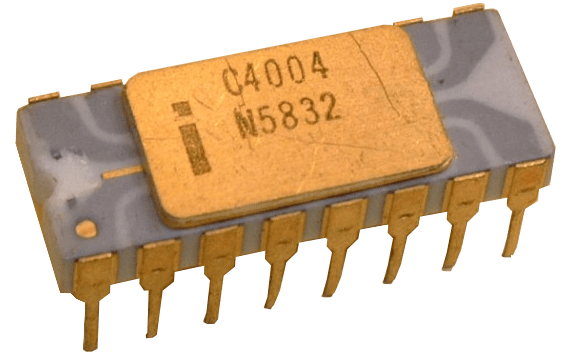
\includegraphics[width=0.45\textwidth]{imagens/intel_4004.png}
\caption{O Intel 4004 (1971), o primeiro microprocessador comercial.}
\end{figure}

Lançado em 1971, o Intel 4004 possuía uma arquitetura de apenas \textbf{4 bits}, um repertório de \textbf{45 instruções} diferentes, e operava a uma frequência de \emph{clock} máxima de \textbf{740 kHz} — para comparação, milhares de vezes mais lento que o \ESP{} que usaremos nesta apostila.

Um microprocessador sozinho, porém, não é suficiente para compor um circuito integrado completo para aplicações embarcadas: ele ainda precisaria de chips externos de memória e de interface para ser útil. Foi para resolver essa lacuna que surgiram os \textbf{microcontroladores} — circuitos integrados que reúnem, em um único chip:

\begin{itemize}
    \item a \textbf{ROM} (\emph{Read-Only Memory}), associada às instruções do programa;
    \item a \textbf{RAM} (\emph{Random-Access Memory}), associada aos dados manipulados durante a execução;
    \item registradores digitais de \textbf{interface} com dispositivos externos — os pinos GPIO e periféricos apresentados no \cref{cap:embarcados}.
\end{itemize}

Esse é, essencialmente, o mesmo modelo — bastante amadurecido e miniaturizado — que encontramos hoje dentro do \ESP{}.

\section{A unidade de processamento}

A \textbf{unidade de processamento} (ou simplesmente \emph{processador}) é o centro de um microcontrolador: é ela quem coordena, executa e gerencia todos os recursos disponíveis. Do ponto de vista da eletrônica digital, essa unidade é um \textbf{circuito sequencial} — ou seja, seu \textbf{estado atual} combinado aos \textbf{dados de entrada} determina qual será o \textbf{próximo estado} que o circuito assumirá.

Essas transições de estado acontecem de forma \textbf{síncrona}, ritmadas por um sinal elétrico periódico chamado \textbf{\emph{clock}}. O intervalo de tempo entre duas transições consecutivas é chamado de \textbf{ciclo}.

\begin{figure}[h]
\centering
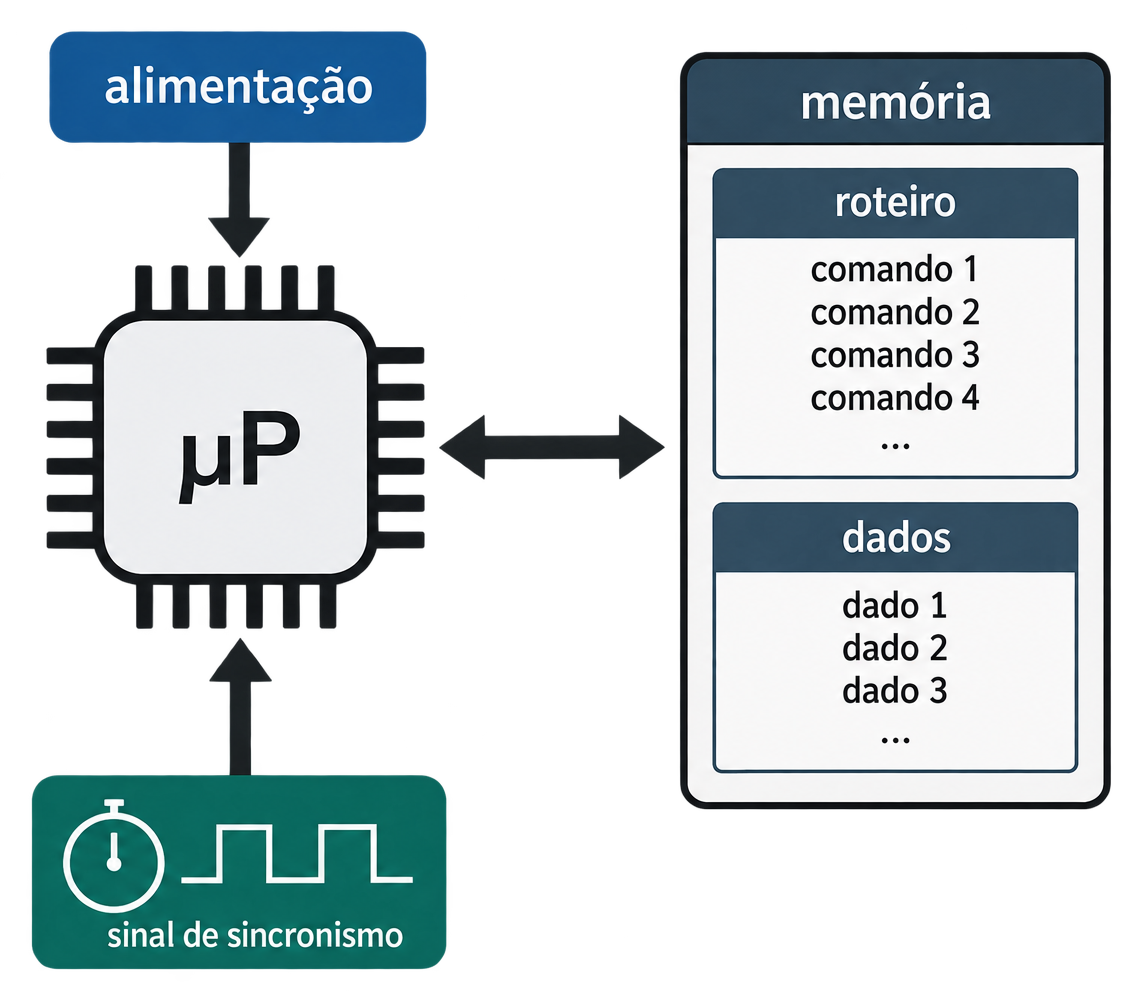
\includegraphics[width=0.72\textwidth]{imagens/estado_microcontrolador.png}
\caption{Visão simplificada de uma unidade de processamento ($\mu$P): alimentação, sinal de sincronismo (\emph{clock}) e o barramento bidirecional de acesso à memória, contendo o roteiro de instruções e os dados do programa.}
\end{figure}

Em cada ciclo, o processador busca a próxima instrução do \textbf{roteiro} (o programa, armazenado na memória de instruções), interpreta o que ela pede para fazer, e a executa — lendo ou escrevendo \textbf{dados}, atualizando registradores, ou desviando para outra instrução. É exatamente essa sequência de busca-decodificação-execução, repetida indefinidamente a cada ciclo de \emph{clock}, que dá vida ao código C que escrevemos: cada linha do seu programa, depois de compilada, se transforma em uma ou mais dessas instruções elementares.

\begin{nota}
Um aprofundamento completo sobre o projeto interno de processadores — unidades de controle, bancos de registradores, pipelines — foge do escopo desta apostila introdutória, mas é um tema fascinante para quem quiser entender ainda melhor o que acontece ``por baixo'' do código C.
\end{nota}

\section{Arquitetura de laço único (\emph{Super Loop})}
\label{sec:super-loop}

Com o hardware entendido em linhas gerais, resta uma pergunta: como \emph{organizar} o firmware que roda sobre ele? A resposta mais simples — e, ainda hoje, a mais usada em projetos de pequeno e médio porte — é a chamada \textbf{arquitetura de laço único} (em inglês, \emph{Super Loop} ou \emph{bare-metal loop}).

A ideia é direta: o firmware é dividido em duas fases.

\begin{enumerate}
    \item Uma fase de \textbf{inicialização}, executada uma única vez, ao ligar o dispositivo — configurar pinos, iniciar periféricos, preparar variáveis;
    \item Um \textbf{laço infinito}, executado indefinidamente depois disso, dentro do qual todas as tarefas do sistema são verificadas e atualizadas repetidamente, uma volta atrás da outra, para sempre.
\end{enumerate}

Você já reconhece essa estrutura: é exatamente o par \code{setup()} / \code{loop()} do framework Arduino, apresentado no \cref{cap:anatomia}. \code{setup()} é a fase de inicialização; \code{loop()}, chamada repetidamente pelo próprio framework, é o laço único.

A grande vantagem da arquitetura de laço único é a \textbf{simplicidade}: não há troca de contexto entre tarefas, não há concorrência para gerenciar, e o comportamento do sistema é fácil de prever e depurar — a cada volta do laço, o código roda sempre na mesma ordem. É também extremamente econômica em termos de memória, o que a torna ideal para microcontroladores simples.

O preço dessa simplicidade é que \textbf{nenhuma tarefa pode bloquear o laço por muito tempo}. Se uma única iteração de \code{loop()} demorar demais — por exemplo, presa em um \code{delay()} longo ou esperando um sensor lento —, \emph{todo} o resto do sistema fica paralisado durante esse tempo: nenhum outro sensor é lido, nenhum outro botão é verificado. É exatamente por isso que o \cref{cap:interrupcoes} apresenta a técnica de temporização por \code{millis()} como alternativa ao \code{delay()} dentro de um laço com múltiplas responsabilidades — e é para proteger o sistema quando, apesar de tudo, alguma tarefa trava por completo, que existe o mecanismo apresentado a seguir.

\section{Watchdog Timer}
\label{sec:watchdog}

Mesmo em um firmware bem projetado, coisas dão errado: um sensor pode parar de responder e travar uma leitura que deveria ser rápida, um laço de espera pode nunca satisfazer sua condição de saída, ou um bug qualquer pode prender a execução em um ponto do código do qual ela nunca retorna. Em uma arquitetura de laço único (\cref{sec:super-loop}), isso é particularmente grave: se \code{loop()} trava, \textbf{o sistema inteiro trava} — sem um sistema operacional completo para intervir, nada tira o processador desse estado sozinho.

A solução para esse problema é um pequeno circuito de hardware chamado \textbf{Watchdog Timer} (WDT, ou ``temporizador de vigilância''): um contador regressivo independente que, se não for \textbf{reiniciado periodicamente pelo próprio firmware}, entende que o sistema travou e força um \textbf{reset} completo do microcontrolador — trazendo-o de volta a um estado conhecido e funcional, em vez de deixá-lo preso indefinidamente.

O uso típico segue um padrão de três passos:

\begin{enumerate}
    \item \textbf{Configurar} o watchdog com um tempo limite (\emph{timeout}) — por exemplo, 5 segundos;
    \item Dentro do laço principal, \textbf{alimentar} (``dar comida a'') o watchdog periodicamente, sempre que o firmware sabe que está funcionando normalmente — isso reinicia a contagem regressiva;
    \item Se, por qualquer motivo, o firmware travar e parar de alimentar o watchdog, o tempo limite se esgota e o \textbf{chip reinicia sozinho}.
\end{enumerate}

\begin{codigoc}{src/main.cpp — protegendo o laço principal com o watchdog}
#include <esp_task_wdt.h>

#define WDT_TIMEOUT 5   // segundos ate o reset, caso nao seja alimentado

void setup() {
    Serial.begin(115200);

    esp_task_wdt_init(WDT_TIMEOUT, true);   // true: reinicia o chip ao vencer
    esp_task_wdt_add(NULL);                 // registra a tarefa de loop() no watchdog

    Serial.println("Watchdog configurado. Sistema iniciado.");
}

void loop() {
    // ... leitura de sensores, logica do programa, etc ...

    Serial.println("Laco em execucao normal.");
    esp_task_wdt_reset();   // "alimenta" o watchdog: avisa que o laco esta vivo

    delay(1000);
}
\end{codigoc}

\begin{dica}
Para ver o watchdog em ação, tente comentar a linha \code{esp\_task\_wdt\_reset();} e substituir o \code{delay(1000)} por um laço vazio bem mais longo que o \code{WDT\_TIMEOUT} configurado (por exemplo, \code{while (true) \{\}}). Poucos segundos depois, o watchdog vai perceber que o laço parou de ser alimentado e reiniciar o \ESP{} sozinho — o monitor serial mostrará a mensagem \code{"Sistema iniciado."} aparecendo repetidamente, uma prova visível de que o mecanismo de proteção está funcionando.
\end{dica}

\begin{atencao}
Chamar \code{esp\_task\_wdt\_reset()} em um ponto do código onde, na verdade, algo já está errado — por exemplo, dentro de um laço de espera que deveria ter um limite de tentativas — \textbf{mascara o problema} em vez de resolvê-lo: o watchdog nunca vai disparar, mesmo que o sistema esteja preso ali, inútil, indefinidamente. O watchdog deve alimentar-se a partir de um ponto do código que só é alcançado quando o laço principal de fato completou uma volta inteira e saudável — nunca de dentro de uma espera que já é, ela própria, suspeita.
\end{atencao}

Com o histórico e a arquitetura de um microcontrolador em mente, o próximo capítulo coloca a mão na massa: a instalação e configuração do \textbf{PlatformIO}, o ambiente que usaremos para escrever, compilar e carregar firmware no \ESP{}.

\chapter[PlatformIO: Ambiente de Desenvolvimento]{PlatformIO:\\Ambiente de Desenvolvimento}
\label{cap:platformio}

Para compilar e carregar código C no \ESP{}, precisamos de uma ferramenta capaz de: (1) compilar o código usando uma \textbf{toolchain cruzada} (o compilador roda no seu computador, mas gera código para o processador Xtensa do \ESP{}, como adiantado no \cref{cap:sistemas-numericos}); (2) transferir o binário resultante para a memória flash do dispositivo via USB; e (3) abrir um canal de comunicação serial para depuração. O \textbf{PlatformIO} faz as três coisas — e muito mais — de forma integrada e gratuita.

\section{O que é o PlatformIO}

PlatformIO é um ecossistema de desenvolvimento profissional para sistemas embarcados, disponível como extensão para o Visual Studio Code (a forma mais comum de uso, e a que seguiremos aqui) ou como ferramenta de linha de comando independente. Ele suporta centenas de placas diferentes — não apenas as placas \ESP{} — e múltiplos \textbf{frameworks} de desenvolvimento para cada uma.

\begin{nota}
Um \textbf{framework}, no contexto do PlatformIO, é o conjunto de bibliotecas e convenções sobre as quais o firmware é escrito. Para o \ESP{}, os dois frameworks mais usados são o \textbf{ESP-IDF} (\emph{Espressif IoT Development Framework}, o SDK oficial da Espressif, escrito em C puro) e o \textbf{Arduino} — uma camada de conveniência sobre esse mesmo SDK, com uma API muito mais simples e enxuta, e o padrão de fato para projetos de prototipagem e IoT. É o framework \textbf{Arduino} que usaremos em todos os exemplos desta apostila daqui em diante.
\end{nota}

\begin{atencao}
Um detalhe técnico importante: arquivos do framework Arduino são compilados como \textbf{C++}, não C puro — é o que permite, por exemplo, que \code{Serial.print(...)} funcione (\code{Serial} é um objeto). Ainda assim, o estilo de código ensinado nesta apostila permanece deliberadamente próximo do C ``puro'' apresentado na Parte I — sem classes, templates ou os demais recursos exclusivos de C++ —, de modo que tudo o que você já aprendeu continua diretamente aplicável. Você vai reconhecer, na prática, que programar para o \ESP{} com Arduino é escrever C dentro de um ambiente C++ minimalista.
\end{atencao}

\section{Instalação}

\begin{enumerate}
    \item Instale o \href{https://code.visualstudio.com/}{Visual Studio Code} (disponível para Windows, macOS e Linux);
    \item Dentro do VS Code, abra a aba de \textbf{Extensões} (ícone de blocos no menu lateral, ou \code{Ctrl+Shift+X});
    \item Busque por \textbf{``PlatformIO IDE''} e clique em \textbf{Instalar};
    \item Aguarde a instalação terminar — na primeira vez, o PlatformIO baixa e configura suas próprias dependências (Python, toolchains de compilação), o que pode levar alguns minutos;
    \item Reinicie o VS Code quando solicitado. Um novo ícone de ``formiga'' (a logo do PlatformIO) deve aparecer na barra lateral esquerda.
\end{enumerate}

\begin{dica}
Não é necessário instalar o Python ou qualquer toolchain manualmente — a extensão do PlatformIO cuida de todo esse processo de forma isolada do restante do sistema, evitando conflitos com outras instalações que você já possa ter.
\end{dica}

\section{Criando um novo projeto}

Com a extensão instalada, clique no ícone da formiga na barra lateral para abrir o \textbf{PIO Home}, e em seguida em \textbf{New Project}. O assistente solicita quatro informações:

\begin{table}[h]
\centering
\begin{tabular}{@{}ll@{}}
\toprule
\textbf{Campo} & \textbf{Valor sugerido} \\
\midrule
Name      & \code{meu-primeiro-projeto} (ou o nome que preferir) \\
Board     & \code{Espressif ESP32 Dev Module} (ajuste conforme sua placa) \\
Framework & \code{Arduino} \\
Location  & a pasta onde o projeto será criado \\
\bottomrule
\end{tabular}
\caption{Configuração do assistente de novo projeto do PlatformIO.}
\end{table}

\begin{atencao}
O campo \textbf{Board} precisa corresponder (ou ao menos ser compatível com) a placa física que você possui. Existem dezenas de variantes de placas baseadas no \ESP{} (DevKit V1, WROOM-32, NodeMCU-32S, entre outras) — quando em dúvida, \code{Espressif ESP32 Dev Module} é uma escolha segura e amplamente compatível para as placas de desenvolvimento mais comuns.
\end{atencao}

\section{Anatomia de um projeto PlatformIO}

Ao criar o projeto, o PlatformIO gera automaticamente a seguinte estrutura de pastas:

\begin{codigoini}{Estrutura de pastas de um projeto PlatformIO}
meu-primeiro-projeto/
|-- platformio.ini      # arquivo de configuracao do projeto
|-- src/                # codigo-fonte principal do firmware
|   `-- main.cpp
|-- include/             # cabecalhos (.h) proprios do projeto
|-- lib/                 # bibliotecas privadas do projeto
`-- test/                # testes automatizados (opcional)
\end{codigoini}

\begin{itemize}
    \item \code{src/} — onde vive o código-fonte principal. É aqui que criaremos e editaremos \code{main.cpp} em todos os exemplos seguintes (a extensão \code{.cpp}, e não \code{.c}, é exigida pelo framework Arduino, como visto na nota anterior);
    \item \code{include/} — para cabeçalhos (\code{.h}) específicos do seu projeto, como os vistos no \cref{cap:modularizacao};
    \item \code{lib/} — para bibliotecas próprias, reutilizáveis entre projetos, ou de terceiros adicionadas manualmente;
    \item \code{platformio.ini} — o coração da configuração do projeto, detalhado a seguir.
\end{itemize}

\subsection{O arquivo \code{platformio.ini}}

\begin{codigoini}{platformio.ini}
[env:esp32dev]
platform = espressif32
board = esp32dev
framework = arduino
monitor_speed = 115200
\end{codigoini}

\begin{table}[h]
\centering
\begin{tabular}{@{}ll@{}}
\toprule
\textbf{Chave} & \textbf{Significado} \\
\midrule
\code{platform}       & a plataforma de hardware (\code{espressif32}, para toda a família \ESP{}) \\
\code{board}          & o identificador exato da placa de desenvolvimento \\
\code{framework}      & o SDK usado (\code{arduino}, nesta apostila) \\
\code{monitor\_speed} & a velocidade (\emph{baud rate}) do monitor serial, em bits por segundo \\
\bottomrule
\end{tabular}
\caption{Principais chaves de configuração do \code{platformio.ini}.}
\end{table}

Esse arquivo texto simples — versionável junto ao código-fonte em um sistema como Git — é o que torna um projeto PlatformIO totalmente reprodutível em qualquer máquina: qualquer pessoa que clone o projeto e abra a pasta no VS Code com a extensão instalada terá exatamente o mesmo ambiente de compilação, sem precisar configurar nada manualmente.

\section{A barra de tarefas do PlatformIO}

Na parte inferior da janela do VS Code, a extensão adiciona uma barra de ícones com as ações mais usadas:

\begin{table}[h]
\centering
\begin{tabular}{@{}ll@{}}
\toprule
\textbf{Ícone} & \textbf{Ação} \\
\midrule
\faCheck\ (visto)         & \textbf{Build} — compila o projeto, sem carregá-lo na placa \\
\faArrowRight\ (seta)     & \textbf{Upload} — compila e carrega o firmware na placa via USB \\
\faPlug\ (tomada)         & \textbf{Serial Monitor} — abre o monitor serial para ver mensagens do firmware \\
\faTrash\ (lixeira)       & \textbf{Clean} — remove arquivos de compilação anteriores \\
\bottomrule
\end{tabular}
\caption{Principais ações da barra de tarefas do PlatformIO no VS Code.}
\end{table}

\begin{dica}
O botão de \textbf{Upload} já executa o \textbf{Build} automaticamente antes de carregar — não é necessário clicar nos dois separadamente. Durante o upload, muitas placas exigem que se segure um botão físico chamado \textbf{BOOT} (ou \textbf{IO0}) no exato momento em que a transferência começa, para entrar em modo de gravação. Se o upload falhar com um erro de timeout de conexão, essa é a primeira coisa a verificar.
\end{dica}

O próximo capítulo detalha o conteúdo mínimo de \code{src/main.cpp} em um projeto Arduino — o equivalente, no mundo embarcado, ao \code{hello\_world.c} do \cref{cap:primeiros-passos}.

\chapter{Anatomia de um Projeto Arduino}
\label{cap:anatomia}

Com o ambiente configurado, é hora de escrever o primeiro firmware de verdade. Este capítulo dissecta a estrutura mínima de um programa Arduino — o ponto de partida para todos os exemplos do restante da apostila.

\section{As funções \code{setup} e \code{loop}}

Diferente de um programa C convencional, onde tudo começa em \code{main}, um \emph{sketch} Arduino (o nome tradicional dado a um programa nesse framework) é organizado em torno de duas funções obrigatórias:

\begin{codigoc}{src/main.cpp — esqueleto mínimo}
void setup() {
    // executado uma unica vez, ao ligar ou reiniciar o ESP32
}

void loop() {
    // executado repetidamente, para sempre, enquanto houver energia
}
\end{codigoc}

\begin{itemize}
    \item \code{setup()} roda \textbf{uma única vez}, logo após o \ESP{} ser ligado ou reiniciado — é o lugar certo para inicializações: configurar pinos, iniciar a comunicação serial, preparar sensores;
    \item \code{loop()} roda \textbf{repetidamente, para sempre}, chamada automaticamente pelo próprio framework assim que \code{setup()} termina — é aqui que mora a lógica principal do firmware, exatamente o ``laço infinito'' adiantado no \cref{cap:primeiros-passos} e no \cref{cap:repeticao}.
\end{itemize}

\begin{nota}
Por que não uma função \code{main}? Tecnicamente, \emph{existe} uma \code{main} nos bastidores — mas ela pertence ao próprio núcleo do framework Arduino, não ao seu código. Esse \code{main} interno cuida de inicializar o hardware e então chama \code{setup()} uma vez, seguida de \code{loop()} dentro de um laço infinito escondido de você. É por isso que \code{setup} e \code{loop} não retornam nenhum valor (\code{void}) e não recebem parâmetros: elas não são o ponto de entrada do programa, apenas dois pontos de extensão que o framework chama em momentos específicos.
\end{nota}

\section{Um primeiro exemplo completo}

\begin{codigoc}{src/main.cpp — contador com atraso}
void setup() {
    Serial.begin(115200);   // inicia a comunicacao serial
}

void loop() {
    static int contador = 0;

    Serial.print("Contador: ");
    Serial.println(contador);
    contador++;

    delay(1000);   // pausa de 1000 ms antes da proxima iteracao
}
\end{codigoc}

\begin{atencao}
A pausa acima usa \code{delay(ms)}, a função padrão do Arduino para aguardar um intervalo de tempo em milissegundos — \textbf{não} um laço vazio de espera ocupada (\emph{busy-waiting}, como \code{for (long i = 0; i < 1000000; i++);}). Por baixo dos panos, o \ESP{} roda sobre um sistema operacional de tempo real (o FreeRTOS, adiantado no \cref{cap:embarcados}), que depende de que cada tarefa devolva o controle periodicamente; \code{delay()} já faz isso de forma segura, permitindo que outras tarefas do sistema (como a pilha de Wi-Fi) continuem funcionando durante a espera. Um laço vazio, em vez disso, prende o processador e pode disparar o \textbf{Watchdog Timer} — o mecanismo de segurança apresentado no \cref{sec:watchdog}, que reinicia o chip sozinho quando percebe que o laço principal ``travou''.
\end{atencao}

\section{Compilando, carregando e monitorando}

Com o código acima salvo em \code{src/main.cpp}, o fluxo de trabalho no PlatformIO é:

\begin{enumerate}
    \item Conecte o \ESP{} ao computador via cabo USB;
    \item Clique no ícone de \textbf{Upload} (\cref{cap:platformio}) — o PlatformIO compila o projeto e carrega o binário na placa;
    \item Clique no ícone de \textbf{Serial Monitor} para ver a saída de \code{Serial.print}/\code{Serial.println} em tempo real.
\end{enumerate}

\begin{codigobash}{Saída esperada no monitor serial}
Contador: 0
Contador: 1
Contador: 2
\end{codigobash}

\begin{dica}
Se o monitor serial mostrar apenas caracteres ilegíveis (``lixo''), a causa quase sempre é uma incompatibilidade entre a velocidade configurada no monitor e a velocidade passada para \code{Serial.begin()} no código. Confirme que \code{monitor\_speed} no \code{platformio.ini} coincide com o valor usado em \code{Serial.begin(...)} — nesta apostila, sempre \code{115200}.
\end{dica}

\section{De volta aos fundamentos: o que você já sabe aplicar}

Vale parar um momento para notar que tudo neste primeiro exemplo já foi visto na Parte I: uma variável \code{static} preservando seu valor entre chamadas (\cref{cap:funcoes}), incremento com \code{++} (\cref{cap:tipos}), e duas funções sem retorno (\code{void}, \cref{cap:funcoes}). Programar o \ESP{} não introduz uma linguagem nova — introduz um \textbf{framework} novo, com suas próprias funções e convenções, construído sobre exatamente o C que você já domina.

Os próximos capítulos exploram, um a um, os periféricos mais importantes do \ESP{}: entradas e saídas digitais (\cref{cap:gpio}), leitura de sensores analógicos (\cref{cap:adc}), comunicação serial (\cref{cap:serial}) e interrupções (\cref{cap:interrupcoes}).

\chapter{Entradas e Saídas Digitais (GPIO)}
\label{cap:gpio}

GPIO (\emph{General Purpose Input/Output}) são os pinos de propósito geral de um microcontrolador — a interface mais básica e mais usada entre o firmware e o mundo físico. Cada pino GPIO pode ser configurado por software como \textbf{saída} (o chip impõe um nível de tensão sobre ele — ligado ou desligado) ou como \textbf{entrada} (o chip lê o nível de tensão presente nele, imposto por algum circuito externo, como um botão).

\begin{esp32box}
O \ESP{} tem várias dezenas de pinos GPIO, numerados (por exemplo, 2, 4, 5, \ldots{} 23). Nem todos podem ser usados livremente: alguns são reservados para a memória flash interna e não devem ser manipulados, outros têm comportamento especial ao ligar (\emph{strapping pins}) e podem interferir no boot se conectados incorretamente. Consulte sempre o \emph{datasheet} ou o diagrama de pinos (\emph{pinout}) da sua placa específica antes de escolher quais pinos usar.
\end{esp32box}

\section{Configurando um pino como saída: o LED}

O exemplo mais tradicional de programação embarcada — o equivalente ao \emph{Hello, World!} — é piscar um LED, o chamado \textbf{blink}.

\begin{codigoc}{src/main.cpp — blink}
#define PINO_LED 2

void setup() {
    pinMode(PINO_LED, OUTPUT);
}

void loop() {
    digitalWrite(PINO_LED, HIGH);   // liga o LED
    delay(500);

    digitalWrite(PINO_LED, LOW);    // desliga o LED
    delay(500);
}
\end{codigoc}

Três funções do Arduino fazem todo o trabalho:

\begin{itemize}
    \item \code{pinMode(pino, modo)} — define se o pino é \code{OUTPUT} (saída) ou \code{INPUT} (entrada), chamada uma única vez em \code{setup()};
    \item \code{digitalWrite(pino, nivel)} — em modo saída, impõe o nível lógico \code{HIGH} (ligado, 3,3~V) ou \code{LOW} (desligado, 0~V);
    \item \code{delay(ms)} — pausa a execução pelo número de milissegundos indicado, como visto no \cref{cap:anatomia}.
\end{itemize}

\begin{atencao}
Os pinos GPIO do \ESP{} operam em \textbf{3,3~V}, não em 5~V como muitas placas Arduino clássicas (como o Arduino Uno). Conectar um sinal de 5~V diretamente a um pino GPIO pode danificar permanentemente o chip. Sempre verifique o nível de tensão de qualquer módulo externo antes de conectá-lo.
\end{atencao}

\section{Configurando um pino como entrada: o botão}

Ler o estado de um botão segue a mesma lógica, com a direção invertida:

\begin{codigoc}{Lendo um botão com resistor de pull-up interno}
#define PINO_LED    2
#define PINO_BOTAO  15

void setup() {
    pinMode(PINO_LED, OUTPUT);
    pinMode(PINO_BOTAO, INPUT_PULLUP);   // resistor de pull-up interno
}

void loop() {
    bool pressionado = (digitalRead(PINO_BOTAO) == LOW);
    // com pull-up, o pino le LOW quando o botao conecta o pino ao GND

    digitalWrite(PINO_LED, pressionado);
    delay(20);   // pequena pausa (debounce simples)
}
\end{codigoc}

\begin{nota}
Um botão simples, ligado entre um pino GPIO e o terra (GND), deixa o pino em um estado \textbf{flutuante} (indefinido) quando não está sendo pressionado, a menos que exista um resistor conectando-o a um nível de tensão conhecido. O modo \code{INPUT\_PULLUP} ativa um resistor de \emph{pull-up} interno ao próprio chip, eliminando a necessidade de um resistor externo para esse caso comum: o pino lê \code{HIGH} quando o botão está solto, e \code{LOW} quando pressionado (conectando o pino ao GND).
\end{nota}

\begin{dica}
Botões mecânicos produzem múltiplas transições elétricas rápidas e espúrias no instante em que são pressionados ou soltos — um fenômeno chamado \emph{bounce}. Um pequeno atraso após cada leitura, como o \code{delay(20)} do exemplo, é uma forma simples (ainda que rudimentar) de filtrar esse ruído, chamada \emph{debouncing}. O \cref{cap:interrupcoes} apresenta uma abordagem mais robusta, baseada em interrupções.
\end{dica}

\section{Controlando vários pinos com um vetor}

Quando um projeto usa vários pinos com o mesmo papel — por exemplo, uma fileira de LEDs —, vale a pena aplicar o que vimos no \cref{cap:arranjos}: guardar os números dos pinos em um \textbf{vetor} e percorrê-lo com um laço, em vez de repetir o mesmo código uma vez para cada pino.

\begin{codigoc}{Controlando vários LEDs com um vetor}
const int pinos_leds[] = {2, 4, 5, 18};
const int quantidade = 4;

void setup() {
    for (int i = 0; i < quantidade; i++) {
        pinMode(pinos_leds[i], OUTPUT);
    }
}

void loop() {
    // acende um LED de cada vez, em sequencia (efeito "corrente")
    for (int i = 0; i < quantidade; i++) {
        digitalWrite(pinos_leds[i], HIGH);
        delay(150);
        digitalWrite(pinos_leds[i], LOW);
    }
}
\end{codigoc}

Além de evitar repetição, essa abordagem torna o código mais fácil de estender: adicionar um quinto LED exige apenas um novo número no vetor \code{pinos\_leds} (e ajustar \code{quantidade}), sem tocar no restante da lógica.

\chapter{Leitura de Sensores Analógicos (ADC)}
\label{cap:adc}

Muitos sensores — potenciômetros, sensores de luminosidade (LDR), sensores de temperatura analógicos — não respondem apenas com ``ligado'' ou ``desligado'': eles produzem uma \textbf{tensão contínua e variável}, proporcional à grandeza física medida. Para ler esse tipo de sinal, usamos um \textbf{ADC} (\emph{Analog-to-Digital Converter}, ou conversor analógico-digital) — a porta de entrada de praticamente todo projeto de monitoramento IoT.

\section{Como um ADC funciona}

Um ADC amostra uma tensão analógica de entrada e a converte em um número inteiro, dentro de uma faixa determinada pela sua \textbf{resolução}, medida em bits. O \ESP{} possui ADCs de \textbf{12 bits}, o que significa que cada leitura retorna um valor entre 0 e $2^{12}-1 = 4095$ — quanto mais próxima a tensão de entrada estiver da tensão máxima suportada, mais próximo de 4095 será o valor lido.

\begin{atencao}
Se você já programou com placas Arduino clássicas (como o Arduino Uno), tenha atenção: lá, \code{analogRead()} retorna valores de \textbf{10 bits} (0 a 1023). No \ESP{}, por padrão, a resolução é de \textbf{12 bits} (0 a 4095) — o dobro de precisão, mas também uma faixa de valores diferente da que você talvez esteja acostumado.
\end{atencao}

\begin{esp32box}
O \ESP{} possui duas unidades ADC independentes: \textbf{ADC1} (8 canais, nos pinos GPIO32 a GPIO39) e \textbf{ADC2} (10 canais, compartilhados com o rádio Wi-Fi — por isso, leituras em ADC2 podem falhar ou ficar imprecisas enquanto o Wi-Fi está ativo). Por essa razão, esta apostila usa exclusivamente pinos da \textbf{ADC1} nos exemplos a seguir.
\end{esp32box}

\begin{table}[h]
\centering
\begin{tabular}{@{}cc@{}}
\toprule
\textbf{Pino GPIO} & \textbf{Unidade ADC} \\
\midrule
GPIO32 & ADC1 \\
GPIO33 & ADC1 \\
GPIO34 & ADC1 \\
GPIO35 & ADC1 \\
GPIO36 & ADC1 \\
GPIO39 & ADC1 \\
\bottomrule
\end{tabular}
\caption{Alguns pinos da ADC1 disponíveis no ESP32.}
\end{table}

\section{Lendo um sensor analógico}

No framework Arduino, uma única função basta para realizar uma leitura: \code{analogRead(pino)}.

\begin{codigoc}{src/main.cpp — lendo um potenciômetro ou LDR}
#define PINO_SENSOR 34

void setup() {
    Serial.begin(115200);
}

void loop() {
    int leitura_bruta = analogRead(PINO_SENSOR);
    float tensao = (leitura_bruta / 4095.0f) * 3.3f;

    Serial.print("Bruto: ");
    Serial.print(leitura_bruta);
    Serial.print("  |  Aproximadamente: ");
    Serial.print(tensao);
    Serial.println(" V");

    delay(500);
}
\end{codigoc}

\begin{atencao}
A conversão \code{(leitura\_bruta / 4095.0f) * 3.3f} usada acima é uma \textbf{aproximação} — assume uma relação perfeitamente linear entre o valor lido e a tensão real, o que não é exatamente verdade na prática devido a não linearidades do hardware do ADC. Para a maioria dos sensores simples em um projeto de aprendizado — um LDR, um potenciômetro, um sensor de temperatura analógico — essa aproximação linear costuma ser suficiente.
\end{atencao}

\section{De leitura bruta a informação: um sensor de luminosidade}

Uma leitura analógica isolada raramente é o objetivo final — o valor bruto do ADC quase sempre precisa ser \textbf{traduzido} para uma grandeza com significado físico, e depois \textbf{registrado} ou \textbf{avaliado}. O exemplo a seguir lê um LDR (fotorresistor), estima um percentual de luminosidade e usa o próprio monitor serial como ferramenta de depuração e acompanhamento — a técnica de \emph{print debugging} apresentada no \cref{cap:entrada-saida}, agora aplicada a um sensor real:

\begin{codigoc}{Estimando luminosidade e registrando via Serial}
#define PINO_LDR 34

void setup() {
    Serial.begin(115200);
}

void loop() {
    int leitura_bruta = analogRead(PINO_LDR);
    float luminosidade_pct = (leitura_bruta / 4095.0f) * 100.0f;

    Serial.print("[SENSOR] LDR bruto=");
    Serial.print(leitura_bruta);
    Serial.print(" luminosidade=");
    Serial.print(luminosidade_pct);
    Serial.println("%");

    if (luminosidade_pct < 20.0f) {
        Serial.println("[ALERTA] Ambiente escuro detectado!");
    }

    delay(1000);
}
\end{codigoc}

\section{Suavizando leituras com um vetor: média móvel}

Sensores analógicos são naturalmente ruidosos — duas leituras consecutivas do mesmo ambiente raramente retornam exatamente o mesmo valor. Uma técnica simples e eficaz para suavizar esse ruído é a \textbf{média móvel}: manter um pequeno histórico das últimas N leituras (usando um vetor, como no \cref{cap:arranjos}) e trabalhar sempre com a média desse histórico, em vez de uma leitura isolada.

\begin{codigoc}{Média móvel das últimas 10 leituras}
#define PINO_SENSOR 34
#define TAMANHO_HISTORICO 10

int historico[TAMANHO_HISTORICO];
int indice_atual = 0;

void setup() {
    Serial.begin(115200);
    for (int i = 0; i < TAMANHO_HISTORICO; i++) {
        historico[i] = 0;
    }
}

void loop() {
    historico[indice_atual] = analogRead(PINO_SENSOR);
    indice_atual = (indice_atual + 1) % TAMANHO_HISTORICO;

    long soma = 0;
    for (int i = 0; i < TAMANHO_HISTORICO; i++) {
        soma += historico[i];
    }
    float media = (float) soma / TAMANHO_HISTORICO;

    Serial.print("[SENSOR] media movel = ");
    Serial.println(media);

    delay(100);
}
\end{codigoc}

O operador \code{\%} (resto da divisão, \cref{cap:tipos}) faz o índice \code{indice\_atual} voltar a 0 automaticamente ao chegar em \code{TAMANHO\_HISTORICO} — o vetor se comporta como um \textbf{buffer circular}, sempre sobrescrevendo a leitura mais antiga com a mais nova. 

\chapter{Comunicação Serial e Depuração}
\label{cap:serial}

Sem teclado, tela ou depurador visual conectado por padrão, a \textbf{comunicação serial} é a principal janela do desenvolvedor para dentro de um firmware em execução — é como saber o que o programa está ``pensando'' a cada momento, essencial tanto para aprender quanto para depurar problemas.

\section{UART e o monitor serial}

O \ESP{} se comunica com o computador através de uma interface \textbf{UART} (\emph{Universal Asynchronous Receiver/Transmitter}), tipicamente ligada a um chip conversor USB-serial na própria placa de desenvolvimento. No framework Arduino, essa comunicação é controlada pelo objeto \code{Serial}, que precisa ser iniciado uma única vez, em \code{setup()}, com a velocidade de comunicação desejada.

\begin{codigoc}{src/main.cpp — contador via Serial}
void setup() {
    Serial.begin(115200);
}

void loop() {
    static int contador = 0;

    Serial.print("Contador: ");
    Serial.println(contador);
    contador++;

    delay(1000);
}
\end{codigoc}

Para visualizar essa saída, use o \textbf{Serial Monitor} do PlatformIO (\cref{cap:platformio}) — ele abre uma conexão serial com a placa na velocidade definida por \code{monitor\_speed} no \code{platformio.ini} (que deve coincidir com o valor passado a \code{Serial.begin}) e exibe, em tempo real, tudo o que o firmware escreve.

\subsection{As variantes de \code{Serial.print}}

\begin{table}[h]
\centering
\begin{tabular}{@{}ll@{}}
\toprule
\textbf{Função} & \textbf{Comportamento} \\
\midrule
\code{Serial.print(x)}     & imprime \code{x}, sem quebra de linha ao final \\
\code{Serial.println(x)}   & imprime \code{x}, seguido de uma quebra de linha \\
\code{Serial.printf(fmt, \ldots)} & imprime com especificadores de formato, como \code{printf} \\
\bottomrule
\end{tabular}
\caption{Formas de escrever na porta serial no framework Arduino.}
\end{table}

\begin{dica}
\code{Serial.printf} aceita exatamente os mesmos especificadores de formato apresentados no \cref{cap:entrada-saida} (\code{\%d}, \code{\%f}, \code{\%s}, \code{\%.2f}, e assim por diante) — todo aquele conhecimento é diretamente reaproveitável aqui, bastando trocar \code{printf(...)} por \code{Serial.printf(...)}.
\end{dica}

\section{Saída como ferramenta de depuração, agora no firmware}

A técnica de \emph{print debugging} apresentada no \cref{sec:printf-debug} — imprimir o valor de uma variável em pontos estratégicos do código para entender o comportamento de um programa — se transporta quase sem alterações para o firmware, usando \code{Serial} no lugar de \code{printf}:

\begin{codigoc}{Depurando uma leitura de sensor}
int leitura_bruta = analogRead(PINO_SENSOR);
Serial.print("[DEBUG] leitura_bruta = ");
Serial.println(leitura_bruta);

float tensao = (leitura_bruta / 4095.0f) * 3.3f;
Serial.print("[DEBUG] tensao = ");
Serial.println(tensao);
\end{codigoc}

\section{Log por nível de severidade}

O núcleo Arduino do \ESP{} também oferece um sistema de \textbf{log por nível de severidade} — uma alternativa mais expressiva que \code{Serial.print} puro, com macros que já indicam a gravidade da mensagem:

\begin{codigoc}{Usando as macros de log}
void setup() {
    Serial.begin(115200);
}

void loop() {
    int leitura = analogRead(34);

    log_i("Sistema em operacao normal.");
    if (leitura < 100) {
        log_w("Leitura muito baixa: %d", leitura);
    }
    if (leitura == 0) {
        log_e("Sensor parece desconectado!");
    }

    delay(1000);
}
\end{codigoc}

\begin{table}[h]
\centering
\begin{tabular}{@{}lll@{}}
\toprule
\textbf{Macro} & \textbf{Nível} & \textbf{Uso típico} \\
\midrule
\code{log\_e} & Error   & falhas que impedem o funcionamento normal \\
\code{log\_w} & Warning & situações anormais, mas não fatais \\
\code{log\_i} & Info    & mensagens informativas de operação normal \\
\code{log\_d} & Debug   & detalhes úteis apenas durante desenvolvimento \\
\code{log\_v} & Verbose & o nível mais detalhado, quase sempre desativado \\
\bottomrule
\end{tabular}
\caption{Níveis de log disponíveis no núcleo Arduino do ESP32.}
\end{table}

O nível mínimo de mensagens exibidas é controlado por uma opção de compilação, ajustável diretamente no \code{platformio.ini}:

\begin{codigoini}{platformio.ini com nível de log elevado}
[env:esp32dev]
platform = espressif32
board = esp32dev
framework = arduino
monitor_speed = 115200
build_flags = -DCORE_DEBUG_LEVEL=4   ; 0=Nenhum ... 5=Verbose
\end{codigoini}

\begin{dica}
A grande vantagem de usar \code{log\_x} em vez de \code{Serial.print} puro é justamente essa: o nível mínimo de log pode ser reduzido em uma versão ``de produção'' do firmware (silenciando mensagens de depuração detalhadas) sem precisar remover ou comentar cada chamada manualmente — basta alterar um único número em \code{platformio.ini}.
\end{dica}

\begin{esp32box}
Uma armadilha clássica ao depurar por log em sistemas embarcados: mensagens de log \emph{também} consomem tempo de processamento e, no caso da UART, banda de comunicação limitada. Excesso de logs dentro de um laço executado milhares de vezes por segundo pode, ele próprio, atrasar o firmware o suficiente para mascarar ou até causar o problema que se está tentando diagnosticar — um efeito colateral que vale ter em mente ao decidir onde e com que frequência logar.
\end{esp32box}

\chapter{Interrupções e Temporização}
\label{cap:interrupcoes}

O botão lido no \cref{cap:gpio} foi verificado por \textbf{sondagem} (\emph{polling}): o laço principal pergunta repetidamente, a cada iteração, ``o botão está pressionado agora?''. Essa abordagem é simples, mas tem um custo — o processador gasta tempo verificando um evento que, na maior parte do tempo, ainda não aconteceu. \textbf{Interrupções} resolvem esse problema de forma elegante: em vez de perguntar, o firmware é \emph{avisado} pelo hardware exatamente no instante em que o evento ocorre.

\section{O que é uma interrupção}

Uma \textbf{interrupção} é um mecanismo de hardware que pausa imediatamente o que o processador está fazendo, executa uma função especial chamada \textbf{rotina de tratamento de interrupção} (\emph{Interrupt Service Routine}, ou \textbf{ISR}), e depois retoma exatamente de onde havia parado — tudo de forma transparente ao código que estava em execução.

\begin{atencao}
Uma ISR deve ser \textbf{extremamente curta e rápida}. Ela interrompe literalmente qualquer coisa que estivesse rodando, então mantê-la presa por muito tempo atrasa todo o resto do sistema. A prática recomendada — usada no exemplo a seguir — é: dentro da ISR, apenas \textbf{sinalizar} que o evento ocorreu (atualizando uma variável) e sair; o processamento de fato acontece depois, dentro de \code{loop()}. Chamar \code{Serial.print}, \code{delay}, ou qualquer função ``pesada'' de dentro de uma ISR deve ser evitado.
\end{atencao}

\section{Interrupções de GPIO com \code{attachInterrupt}}

Vamos reescrever a leitura de botão do \cref{cap:gpio}, agora reagindo por interrupção em vez de sondagem.

\begin{codigoc}{src/main.cpp — botão via interrupção}
#define PINO_BOTAO 15

volatile bool evento_botao = false;

void IRAM_ATTR botao_isr() {
    evento_botao = true;   // apenas sinaliza: nada de Serial aqui dentro
}

void setup() {
    Serial.begin(115200);
    pinMode(PINO_BOTAO, INPUT_PULLUP);

    // dispara a ISR na borda de descida (quando o botao e pressionado)
    attachInterrupt(digitalPinToInterrupt(PINO_BOTAO), botao_isr, FALLING);
}

void loop() {
    if (evento_botao) {
        evento_botao = false;   // consome o evento
        Serial.println("Botao foi pressionado!");
    }
}
\end{codigoc}

\begin{itemize}
    \item \code{attachInterrupt(pino, funcao, modo)} registra \code{botao\_isr} para ser chamada automaticamente pelo hardware sempre que o evento especificado ocorrer no pino indicado — \code{digitalPinToInterrupt()} converte o número do pino para o identificador de interrupção correspondente;
    \item \code{FALLING} dispara a interrupção na \textbf{borda de descida} — o instante exato em que o nível do pino cai de alto para baixo (o momento em que um botão com pull-up é pressionado). Outras opções incluem \code{RISING} (borda de subida) e \code{CHANGE} (qualquer mudança de nível);
    \item \code{IRAM\_ATTR} garante que o código da ISR fique carregado na memória RAM interna do \ESP{}, exigido pelo framework para funções chamadas a partir de uma interrupção;
    \item A variável \code{evento\_botao} é declarada \code{volatile} — exatamente pelo motivo explicado no \cref{cap:funcoes}: seu valor é alterado de forma assíncrona pela ISR, e o compilador não pode assumir que ela permanece constante entre uma leitura e outra dentro de \code{loop()}.
\end{itemize}

\begin{dica}
Esse padrão — ISR mínima apenas sinalizando uma variável \code{volatile}, processamento de fato feito depois em \code{loop()} — também resolve o problema de \emph{debounce} do \cref{cap:gpio} de forma mais robusta: é possível ignorar novos eventos por um curto período após o último processado (comparando o tempo decorrido, como veremos a seguir), sem nunca bloquear a interrupção em si.
\end{dica}

\section{Temporização sem bloquear o laço: a técnica de \code{millis()}}

Até aqui, todos os atrasos usaram \code{delay(ms)} — mas \code{delay} \textbf{bloqueia completamente} a execução de \code{loop()} durante aquele intervalo, impedindo que qualquer outra coisa aconteça nesse meio tempo (ler outro sensor, verificar outro botão, atualizar outro dispositivo). Para tarefas periódicas que não podem se dar ao luxo de bloquear o resto do programa, o Arduino oferece a função \code{millis()}, que retorna o número de milissegundos desde que o \ESP{} foi ligado.

\begin{codigoc}{Piscando um LED sem usar delay()}
#define PINO_LED 2
const unsigned long INTERVALO = 1000;   // 1000 ms

unsigned long ultimo_instante = 0;
bool estado_led = false;

void setup() {
    pinMode(PINO_LED, OUTPUT);
}

void loop() {
    unsigned long agora = millis();

    if (agora - ultimo_instante >= INTERVALO) {
        ultimo_instante = agora;
        estado_led = !estado_led;
        digitalWrite(PINO_LED, estado_led);
    }

    // o resto de loop() continua livre para fazer outras coisas
    // a cada volta, sem nunca ficar bloqueado esperando
}
\end{codigoc}

Essa comparação — ``já se passou tempo suficiente desde a última vez?'' — é um padrão tão comum em firmware que tem nome: \textbf{temporização cooperativa} (ou, informalmente, o padrão \emph{blink without delay}). Ao contrário de um \code{delay()}, \code{loop()} continua girando livremente a cada iteração; a ação só acontece quando o tempo decorrido atinge o intervalo desejado, deixando o restante do código livre para tratar sensores, botões e outras tarefas no meio tempo.

\begin{esp32box}
Combinar \textbf{interrupções} (para eventos externos imprevisíveis, como um botão) com \textbf{temporização por \code{millis()}} (para tarefas periódicas e previsíveis, como ler um sensor a cada segundo) é o padrão de projeto mais comum em firmware Arduino para o \ESP{} — e é exatamente essa combinação que usaremos no projeto integrador do próximo capítulo.
\end{esp32box}

\chapter{Estação de Monitoramento IoT}
\label{cap:projeto-final}

Este capítulo final reúne, em um único projeto, praticamente tudo o que foi apresentado nesta apostila: tipos de dados, estruturas de controle, funções, vetores, \code{structs} e \code{enums}, além de GPIO, ADC, comunicação serial e interrupções. O objetivo é consolidar esses conceitos através de um firmware completo e funcional — não apenas um exemplo isolado de cada periférico.

\section{Especificação do projeto}

Uma \textbf{estação de monitoramento} de luminosidade ambiente: o \ESP{} lê continuamente um sensor LDR, mantém uma média móvel das últimas leituras para suavizar ruído, registra o estado do ambiente pela porta serial e acende um LED de alerta sempre que o ambiente estiver escuro. Um botão alterna entre modo \textbf{normal} (só registra alertas) e modo \textbf{verboso} (registra cada leitura) — sem nunca bloquear o laço principal com \code{delay}.

\subsection{Materiais}

\begin{itemize}
    \item 1 placa de desenvolvimento \ESP{};
    \item 1 LED (com resistor limitador em série, \textasciitilde220~$\Omega$), como indicador de alerta;
    \item 1 sensor LDR, em um divisor de tensão com um resistor fixo (\textasciitilde10~k$\Omega$);
    \item 1 botão \emph{push-button};
    \item Protoboard e jumpers.
\end{itemize}

\subsection{Ligações sugeridas}

\begin{itemize}
    \item LED de alerta $\rightarrow$ GPIO2 (através do resistor limitador, ao GND);
    \item Ponto médio do divisor de tensão do LDR $\rightarrow$ GPIO34 (ADC1);
    \item Botão $\rightarrow$ GPIO15 e GND (usando o \emph{pull-up} interno, como no \cref{cap:gpio}).
\end{itemize}

\section{Projetando a estrutura do estado}

Antes de escrever o laço principal, vale modelar o \textbf{estado} do sistema com os tipos vistos no \cref{cap:structs} — uma prática de organização que se torna cada vez mais valiosa à medida que um firmware cresce:

\begin{codigoc}{Modelando o estado do sistema}
enum ModoOperacao {
    MODO_NORMAL,
    MODO_VERBOSO,
};

struct EstadoEstacao {
    ModoOperacao modo;
    int ultima_leitura;
    float media_movel;
    bool alerta_ativo;
};
\end{codigoc}

Agrupar essas variáveis em uma única \code{struct}, em vez de espalhá-las como variáveis globais soltas, deixa explícito o que compõe ``o estado do sistema'' — e facilita, por exemplo, passar esse estado inteiro para uma função de log, caso o projeto cresça no futuro.

\section{Firmware completo}

\begin{codigoc}{src/main.cpp — estação de monitoramento IoT}
#define PINO_LED    2
#define PINO_LDR    34
#define PINO_BOTAO  15

#define TAMANHO_HISTORICO   10
#define LIMIAR_ESCURO       25.0f   // abaixo disso, ambiente "escuro" (%)
#define INTERVALO_LEITURA   500UL   // ms entre leituras do sensor

enum ModoOperacao {
    MODO_NORMAL,
    MODO_VERBOSO,
};

struct EstadoEstacao {
    ModoOperacao modo;
    int ultima_leitura;
    float media_movel;
    bool alerta_ativo;
};

EstadoEstacao estado = {MODO_NORMAL, 0, 0.0f, false};

int historico[TAMANHO_HISTORICO];
int indice_historico = 0;

volatile bool evento_botao = false;
unsigned long ultima_leitura_ms = 0;

void IRAM_ATTR botao_isr() {
    evento_botao = true;
}

float calcular_media(void) {
    long soma = 0;
    for (int i = 0; i < TAMANHO_HISTORICO; i++) {
        soma += historico[i];
    }
    return (float) soma / TAMANHO_HISTORICO;
}

void setup() {
    Serial.begin(115200);

    pinMode(PINO_LED, OUTPUT);
    pinMode(PINO_BOTAO, INPUT_PULLUP);
    attachInterrupt(digitalPinToInterrupt(PINO_BOTAO), botao_isr, FALLING);

    for (int i = 0; i < TAMANHO_HISTORICO; i++) {
        historico[i] = 0;
    }

    Serial.println("Estacao de monitoramento iniciada em modo NORMAL.");
}

void loop() {
    // 1) verifica se o botao foi pressionado (sem bloquear o laco)
    if (evento_botao) {
        evento_botao = false;
        estado.modo = (estado.modo == MODO_NORMAL) ? MODO_VERBOSO : MODO_NORMAL;

        Serial.print("Modo alterado para: ");
        Serial.println(estado.modo == MODO_NORMAL ? "NORMAL" : "VERBOSO");
    }

    // 2) le o sensor periodicamente, sem usar delay()
    unsigned long agora = millis();
    if (agora - ultima_leitura_ms >= INTERVALO_LEITURA) {
        ultima_leitura_ms = agora;

        estado.ultima_leitura = analogRead(PINO_LDR);
        historico[indice_historico] = estado.ultima_leitura;
        indice_historico = (indice_historico + 1) % TAMANHO_HISTORICO;

        estado.media_movel = calcular_media();
        float luminosidade_pct = (estado.media_movel / 4095.0f) * 100.0f;
        estado.alerta_ativo = (luminosidade_pct < LIMIAR_ESCURO);

        digitalWrite(PINO_LED, estado.alerta_ativo);

        if (estado.modo == MODO_VERBOSO) {
            Serial.print("[LEITURA] bruta=");
            Serial.print(estado.ultima_leitura);
            Serial.print(" media=");
            Serial.print(estado.media_movel);
            Serial.print(" luminosidade=");
            Serial.print(luminosidade_pct);
            Serial.println("%");
        }

        if (estado.alerta_ativo) {
            Serial.println("[ALERTA] Ambiente escuro detectado!");
        }
    }
}
\end{codigoc}

\section{Como o projeto se encaixa}

\begin{itemize}
    \item A \code{struct EstadoEstacao} e a \code{enum ModoOperacao} (\cref{cap:structs}) organizam o estado do sistema de forma clara, em vez de espalhá-lo em variáveis globais soltas;
    \item O vetor \code{historico} (\cref{cap:arranjos}) implementa um \textbf{buffer circular} para a média móvel, suavizando o ruído natural do sensor, exatamente como praticado no \cref{cap:adc};
    \item A leitura do LDR usa a \textbf{ADC} (\cref{cap:adc}) para medir luminosidade de forma contínua, convertida de valor bruto para porcentagem com um \emph{cast} (\cref{cap:tipos});
    \item O botão é lido por \textbf{interrupção} (\cref{cap:interrupcoes}), sinalizando o laço principal por meio de uma variável \code{volatile}, sem nunca bloquear a leitura contínua do sensor;
    \item A leitura periódica do sensor usa a técnica de \textbf{temporização por \code{millis()}} (\cref{cap:interrupcoes}), mantendo \code{loop()} sempre livre para reagir ao botão a qualquer momento;
    \item Todo o comportamento é registrado pela \textbf{porta serial} (\cref{cap:serial}) — mensagens de leitura apenas em modo verboso, e alertas sempre, independentemente do modo.
\end{itemize}

\section{Para continuar praticando}

Esta apostila termina aqui, mas o aprendizado de sistemas embarcados é, acima de tudo, prático. Como próximos passos a partir deste projeto, considere:

\begin{itemize}
    \item Adicionar um segundo sensor (por exemplo, um sensor de temperatura) e expandir a \code{struct EstadoEstacao} para incluí-lo;
    \item Salvar o \code{modo} escolhido na memória flash (usando a biblioteca \code{Preferences} do Arduino para ESP32), para que a estação lembre a última configuração mesmo após ser desligada;
    \item Explorar a conectividade Wi-Fi do \ESP{} para reportar as leituras a um servidor ou aplicativo remoto — o próximo passo natural de qualquer projeto de IoT;
    \item Reescrever o projeto dividindo-o em múltiplos arquivos \code{.h}/\code{.cpp} (\cref{cap:modularizacao}) — por exemplo, separando a lógica do sensor, do histórico e do botão em módulos independentes.
\end{itemize}

Cada um desses passos reutiliza e aprofunda os mesmos fundamentos de C apresentados nesta apostila — a linguagem muda pouco; o que cresce é a sua familiaridade com o hardware e o ecossistema ao redor dela.


\appendix
\chapter{Tabela ASCII}
\label{ap:ascii}

A tabela ASCII (\emph{American Standard Code for Information Interchange}) define a correspondência entre valores numéricos inteiros e caracteres — é o que permite que um \code{char} em C seja, ao mesmo tempo, um número e um caractere. Os valores de 0 a 31 são \textbf{caracteres de controle}, não imprimíveis (como \code{\textbackslash n} e \code{\textbackslash t}, vistos no \cref{cap:entrada-saida}).

\begin{table}[h]
\centering
\begin{tabular}{@{}cl@{\hspace{1cm}}cl@{\hspace{1cm}}cl@{\hspace{1cm}}cl@{}}
\toprule
\textbf{Dec} & \textbf{Char} & \textbf{Dec} & \textbf{Char} & \textbf{Dec} & \textbf{Char} & \textbf{Dec} & \textbf{Char} \\
\midrule
32 & (espaço) & 56 & 8 & 80 & P & 104 & h \\
33 & !  & 57 & 9 & 81 & Q & 105 & i \\
34 & "  & 58 & : & 82 & R & 106 & j \\
35 & \#  & 59 & ; & 83 & S & 107 & k \\
36 & \$  & 60 & < & 84 & T & 108 & l \\
37 & \%  & 61 & = & 85 & U & 109 & m \\
38 & \&  & 62 & > & 86 & V & 110 & n \\
39 & '  & 63 & ? & 87 & W & 111 & o \\
40 & (  & 64 & @ & 88 & X & 112 & p \\
41 & )  & 65 & A & 89 & Y & 113 & q \\
42 & *  & 66 & B & 90 & Z & 114 & r \\
43 & +  & 67 & C & 91 & [ & 115 & s \\
44 & ,  & 68 & D & 92 & \textbackslash & 116 & t \\
45 & -  & 69 & E & 93 & ] & 117 & u \\
46 & .  & 70 & F & 94 & \textasciicircum & 118 & v \\
47 & /  & 71 & G & 95 & \_ & 119 & w \\
48 & 0  & 72 & H & 96 & ` & 120 & x \\
49 & 1  & 73 & I & 97 & a & 121 & y \\
50 & 2  & 74 & J & 98 & b & 122 & z \\
51 & 3  & 75 & K & 99 & c & 123 & \{ \\
52 & 4  & 76 & L & 100 & d & 124 & | \\
53 & 5  & 77 & M & 101 & e & 125 & \} \\
54 & 6  & 78 & N & 102 & f & 126 & \textasciitilde \\
55 & 7  & 79 & O & 103 & g & & \\
\bottomrule
\end{tabular}
\caption{Tabela ASCII imprimível (valores decimais 32 a 126).}
\end{table}

\begin{table}[h]
\centering
\begin{tabular}{@{}cll@{}}
\toprule
\textbf{Dec} & \textbf{Nome} & \textbf{Sequência de escape em C} \\
\midrule
0  & NUL (nulo)         & \code{\textbackslash 0} \\
7  & BEL (alarme sonoro) & \code{\textbackslash a} \\
8  & BS (backspace)      & \code{\textbackslash b} \\
9  & TAB (tabulação)     & \code{\textbackslash t} \\
10 & LF (nova linha)     & \code{\textbackslash n} \\
13 & CR (retorno de carro) & \code{\textbackslash r} \\
27 & ESC (escape)        & --- \\
\bottomrule
\end{tabular}
\caption{Caracteres de controle mais relevantes para programação em C.}
\end{table}

\begin{dica}
Como todo caractere é internamente um número, é possível fazer aritmética diretamente sobre \code{char}s. Por exemplo, \code{'a' - 'A'} vale 32 (a diferença de posição entre maiúsculas e minúsculas na tabela), e \code{('a' + 1)} vale \code{'b'} — uma técnica comum para converter maiúsculas em minúsculas ou percorrer o alfabeto em um laço.
\end{dica}

\chapter{Referência Rápida}
\label{ap:referencia}

Este apêndice reúne, em formato de consulta rápida, tabelas já apresentadas ao longo da apostila — útil como cola de referência durante os primeiros projetos, sem precisar percorrer os capítulos inteiros novamente.

\section{Precedência de operadores}

Da maior para a menor precedência (operadores na mesma linha têm precedência igual, avaliados conforme sua associatividade):

\begin{table}[h]
\centering
\begin{tabular}{@{}ll@{}}
\toprule
\textbf{Operadores} & \textbf{Categoria} \\
\midrule
\code{()} \ \code{[]} \ \code{->} \ \code{.}        & chamada, indexação, acesso a membro \\
\code{!} \ \code{\textasciitilde} \ \code{++} \ \code{--} \ \code{(tipo)} \ \code{*} \ \code{\&} \ \code{sizeof} & unários, cast, ponteiro \\
\code{*} \ \code{/} \ \code{\%}                     & multiplicativos \\
\code{+} \ \code{-}                                 & aditivos \\
\code{<<} \ \code{>>}                               & deslocamento de bits \\
\code{<} \ \code{<=} \ \code{>} \ \code{>=}         & relacionais \\
\code{==} \ \code{!=}                               & igualdade \\
\code{\&}                                            & E bit a bit \\
\code{\textasciicircum}                             & OU exclusivo bit a bit \\
\code{|}                                             & OU bit a bit \\
\code{\&\&}                                          & E lógico \\
\code{||}                                            & OU lógico \\
\code{?:}                                            & ternário \\
\code{=} \ \code{+=} \ \code{-=} \ \code{*=} \ldots  & atribuição \\
\code{,}                                             & vírgula \\
\bottomrule
\end{tabular}
\caption{Precedência de operadores em C, do maior para o menor.}
\end{table}

\begin{dica}
Na dúvida sobre a ordem de avaliação de uma expressão complexa, use parênteses explícitos — isso nunca está errado, e deixa a intenção do código clara tanto para o compilador quanto para quem lê depois.
\end{dica}

\section{Especificadores de formato (\code{printf}/\code{scanf})}

\begin{table}[h]
\centering
\begin{tabular}{@{}ll@{}}
\toprule
\textbf{Especificador} & \textbf{Tipo} \\
\midrule
\code{\%d} / \code{\%i} & \code{int} \\
\code{\%u}              & \code{unsigned int} \\
\code{\%ld} / \code{\%lu} & \code{long} / \code{unsigned long} \\
\code{\%f}              & \code{float} / \code{double} \\
\code{\%.Nf}            & ponto flutuante com N casas decimais \\
\code{\%c}              & \code{char} \\
\code{\%s}              & string (\code{char *}) \\
\code{\%x} / \code{\%X} & hexadecimal (minúsculo / maiúsculo) \\
\code{\%o}              & octal \\
\code{\%p}              & endereço de ponteiro \\
\code{\%zu}             & \code{size\_t} (retorno de \code{sizeof}) \\
\bottomrule
\end{tabular}
\caption{Especificadores de formato mais usados.}
\end{table}

\section{Tipos de largura fixa (\code{stdint.h})}

\begin{table}[h]
\centering
\begin{tabular}{@{}lc@{}}
\toprule
\textbf{Tipo} & \textbf{Intervalo} \\
\midrule
\code{uint8\_t}  & 0 a 255 \\
\code{int8\_t}   & $-128$ a 127 \\
\code{uint16\_t} & 0 a 65\,535 \\
\code{int16\_t}  & $-32\,768$ a 32\,767 \\
\code{uint32\_t} & 0 a $2^{32}\!-\!1$ \\
\code{int32\_t}  & $-2^{31}$ a $2^{31}\!-\!1$ \\
\bottomrule
\end{tabular}
\caption{Tipos inteiros de largura fixa.}
\end{table}

\section{Funções essenciais do framework Arduino usadas nesta apostila}

\begin{table}[h]
\centering
\begin{tabular}{@{}ll@{}}
\toprule
\textbf{Função / macro} & \textbf{Finalidade} \\
\midrule
\code{pinMode(pino, modo)}     & define um pino como \code{OUTPUT}, \code{INPUT} ou \code{INPUT\_PULLUP} \\
\code{digitalWrite(pino, nivel)} & escreve nível lógico (\code{HIGH}/\code{LOW}) em um pino de saída \\
\code{digitalRead(pino)}       & lê o nível lógico de um pino de entrada \\
\code{analogRead(pino)}        & realiza uma leitura do ADC (0 a 4095 no \ESP{}) \\
\code{delay(ms)}                & pausa cooperativa, em milissegundos \\
\code{millis()}                 & milissegundos desde a inicialização (para temporização sem bloqueio) \\
\code{Serial.begin(baud)}       & inicia a comunicação serial na velocidade indicada \\
\code{Serial.print} / \code{Serial.println} & escreve na porta serial, com ou sem quebra de linha \\
\code{Serial.printf(fmt, \ldots)} & escrita formatada na porta serial (especificadores de \code{printf}) \\
\code{attachInterrupt(pino, isr, modo)} & associa uma função ISR a um pino (\code{RISING}/\code{FALLING}/\code{CHANGE}) \\
\code{digitalPinToInterrupt(pino)} & converte um número de pino no identificador de interrupção \\
\code{IRAM\_ATTR}               & garante que uma ISR fique carregada na RAM interna \\
\code{log\_i} / \code{log\_w} / \code{log\_e} & mensagens de log por nível de severidade \\
\code{randomSeed} / \code{random} & inicializa a semente e gera números pseudoaleatórios \\
\code{esp\_task\_wdt\_init/add/reset} & configura, registra e alimenta o Watchdog Timer \\
\code{esp\_sleep\_enable\_timer\_wakeup} & configura um temporizador como fonte de despertar \\
\code{esp\_light\_sleep\_start()}      & entra em \emph{light sleep} (RAM preservada, execução retomada) \\
\code{esp\_sleep\_enable\_gpio\_wakeup()} / \code{gpio\_wakeup\_enable} & configura um pino como fonte de despertar do \emph{light sleep} \\
\code{esp\_deep\_sleep\_start()}       & coloca o \ESP{} em modo \emph{deep sleep} \\
\code{RTC\_DATA\_ATTR}                 & preserva uma variável entre ciclos de \emph{deep sleep} \\
\code{WiFi.begin(ssid, senha)}         & inicia a conexão a uma rede Wi-Fi \\
\code{WiFi.status()} / \code{WiFi.localIP()} & consulta o estado da conexão / o IP obtido \\
\code{HTTPClient} (\code{begin}/\code{POST}/\code{end}) & realiza requisições HTTP \\
\code{ArduinoOTA.begin()} / \code{.handle()} & habilita e processa atualizações de firmware pela rede \\
\bottomrule
\end{tabular}
\caption{Funções do framework Arduino apresentadas na Parte II desta apostila.}
\end{table}


\backmatter

\end{document}
